% Diagnostic figures for the best DTW/DDTW configuration of each CEC2022
% function. This is an input fragment for paper/results.tex and requires only
% graphicx, already loaded by the main paper preamble.
%
% Selection criterion: lowest mean objective over the 31-run DTW and DDTW
% campaigns. The paired plots correspond to the best run of that campaign.

Figures~\ref{fig:cec-best-f1}--\ref{fig:cec-best-f12} show the convergence
trajectory and the $\Delta$ monitor for the better alignment variant selected
independently for each CEC2022 function. Since CEC2022 is a minimization
benchmark, the selection uses the lower mean objective over the 31 runs. DTW
is selected for F1, F3, F5--F8, and F11; DDTW is selected for F2, F4, F9,
F10, and F12. Each pair uses the best run reported by the selected
campaign.

\begin{figure}[H]
\centering
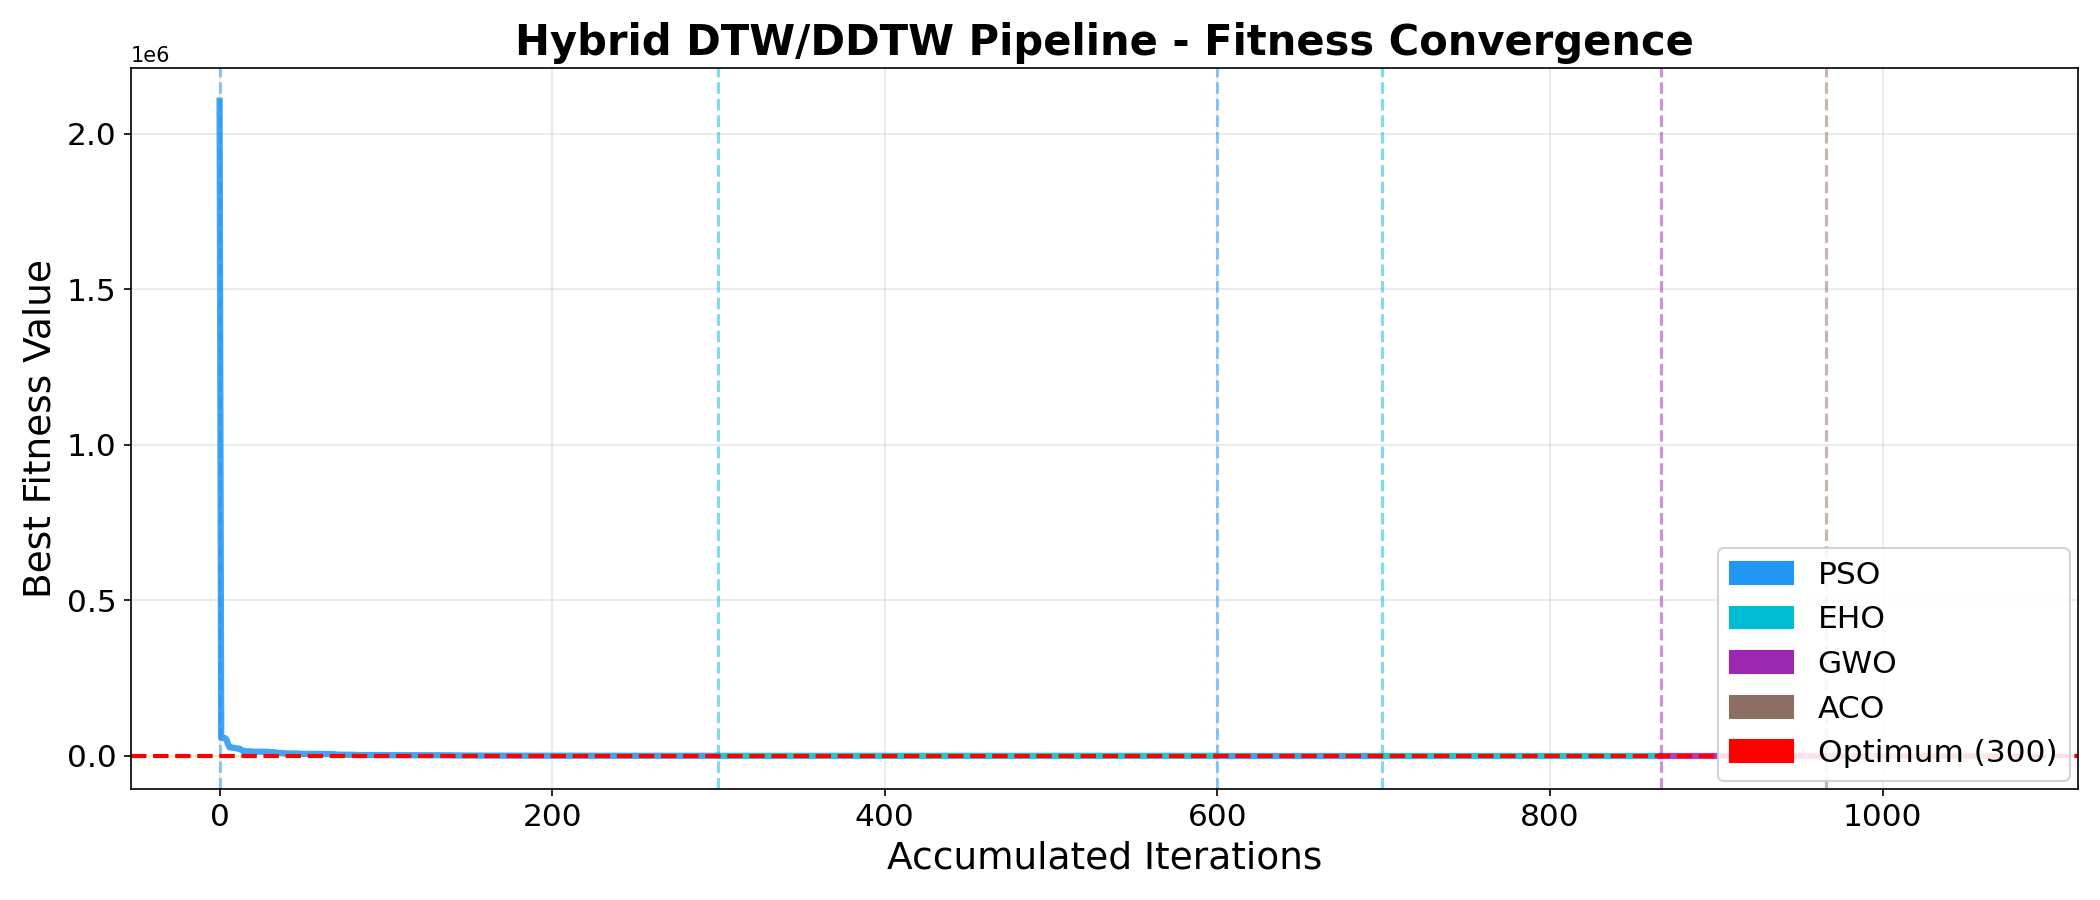
\includegraphics[width=0.7\linewidth]{imagenes_cec_mejores/cec_f1_dtw_convergencia.png}\hfill
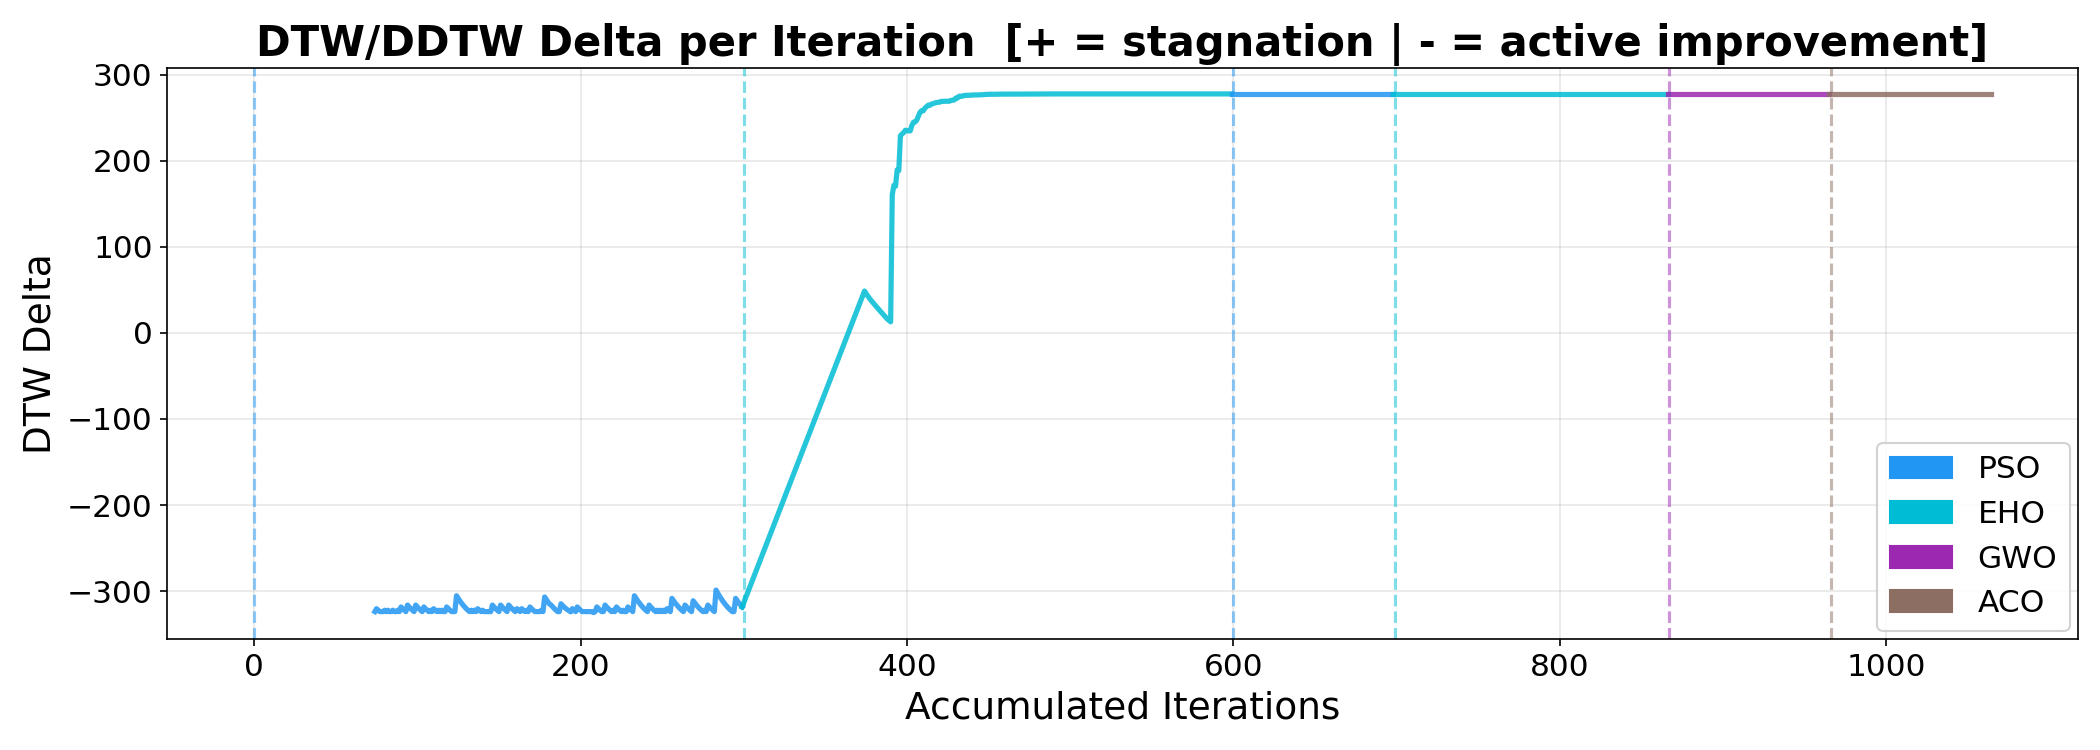
\includegraphics[width=0.7\linewidth]{imagenes_cec_mejores/cec_f1_dtw_dtw_delta.png}
\caption{Convergence trajectory (left) and $\Delta$ monitor (right) for
\texttt{F1} (Shifted Rotated Zakharov) under DTW, best run 09.}
\label{fig:cec-best-f1}
\end{figure}

\begin{figure}[H]
\centering
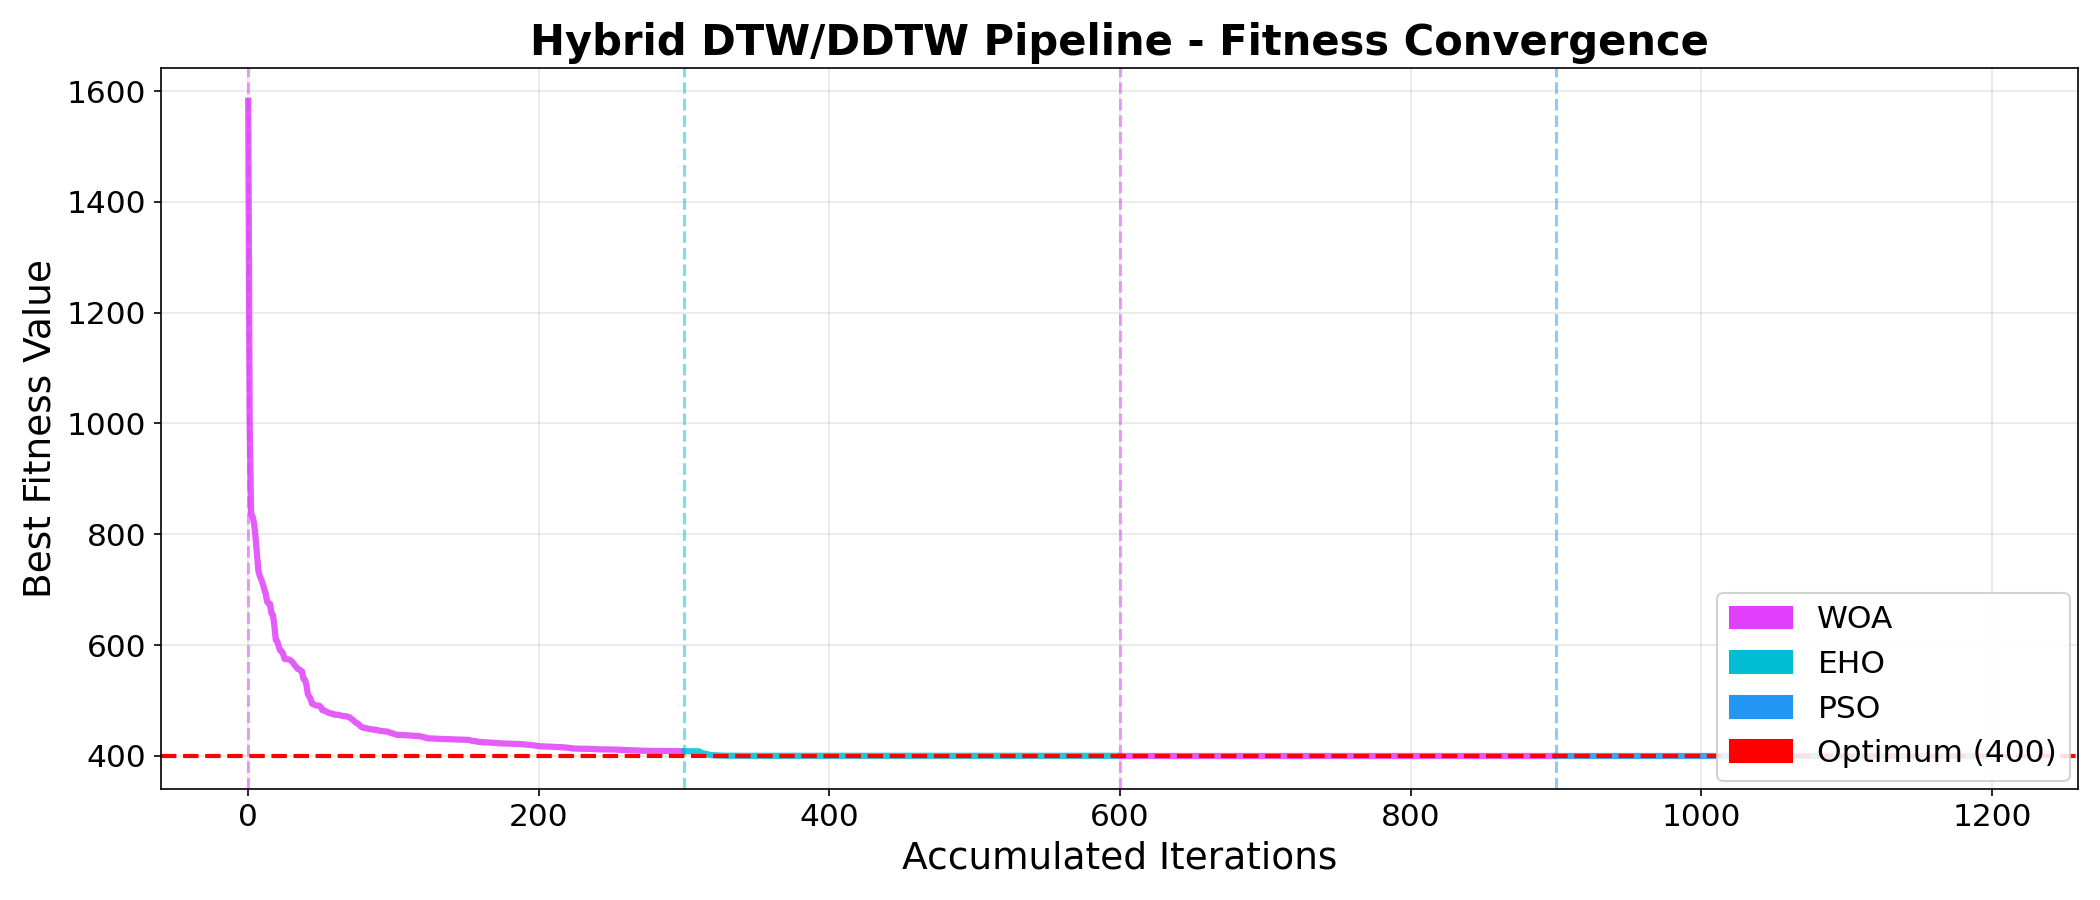
\includegraphics[width=0.7\linewidth]{imagenes_cec_mejores/cec_f2_ddtw_convergencia.png}\hfill
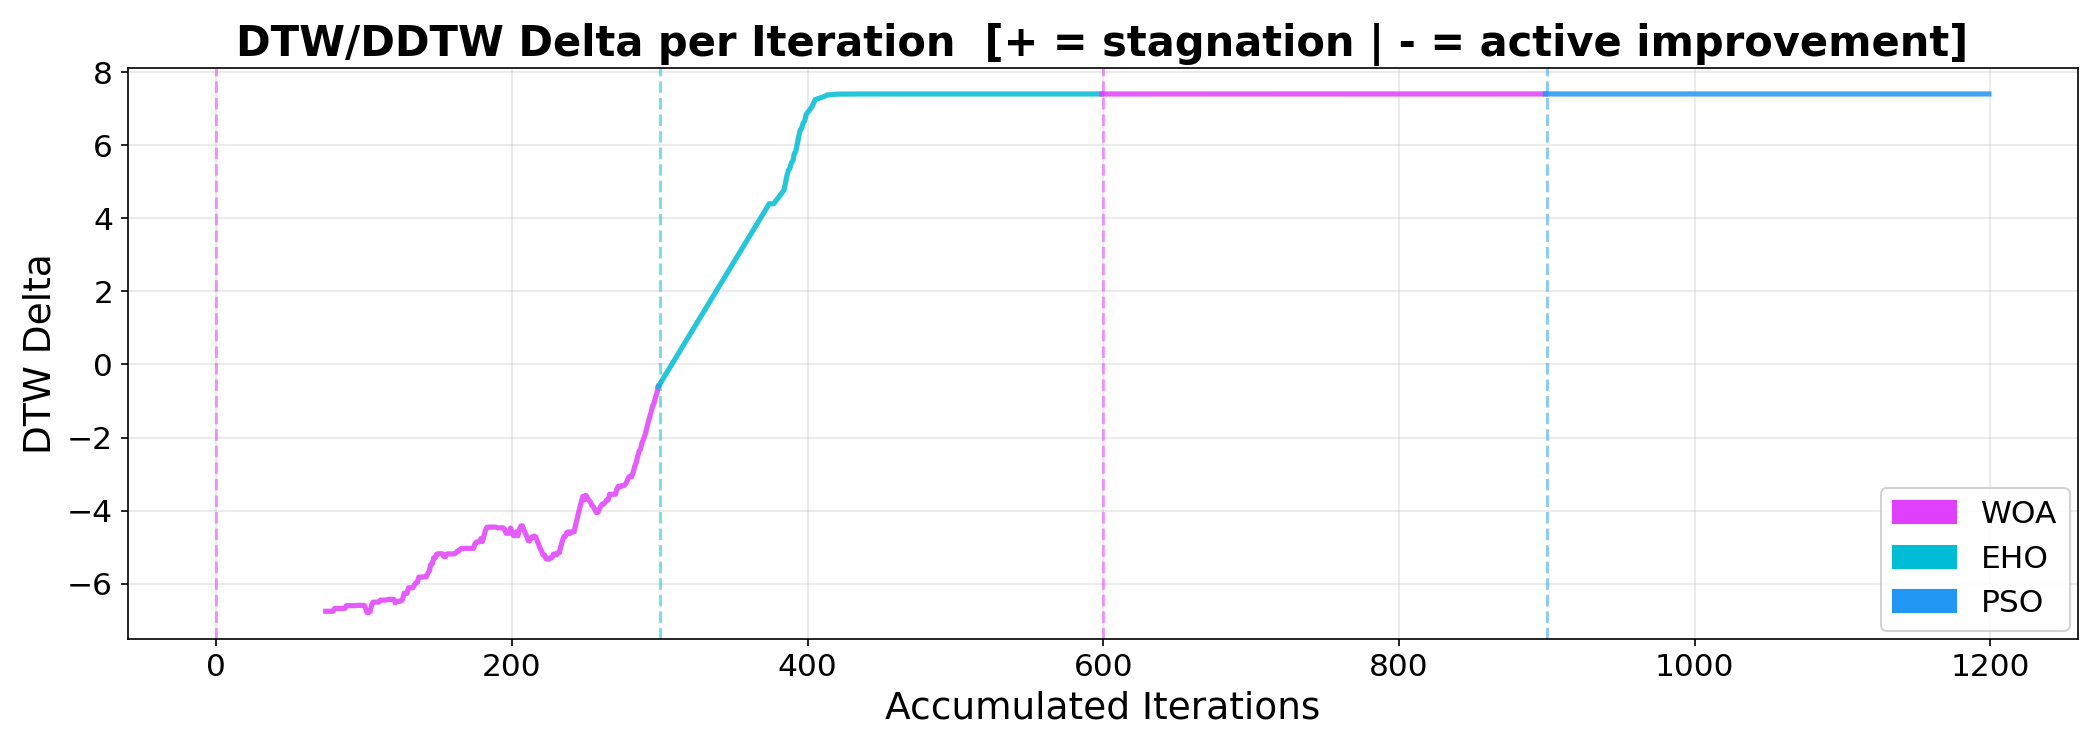
\includegraphics[width=0.7\linewidth]{imagenes_cec_mejores/cec_f2_ddtw_dtw_delta.png}
\caption{Convergence trajectory (left) and $\Delta$ monitor (right) for
\texttt{F2} (Shifted Rotated Rosenbrock) under DDTW, best run 04.}
\label{fig:cec-best-f2}
\end{figure}

\begin{figure}[H]
\centering
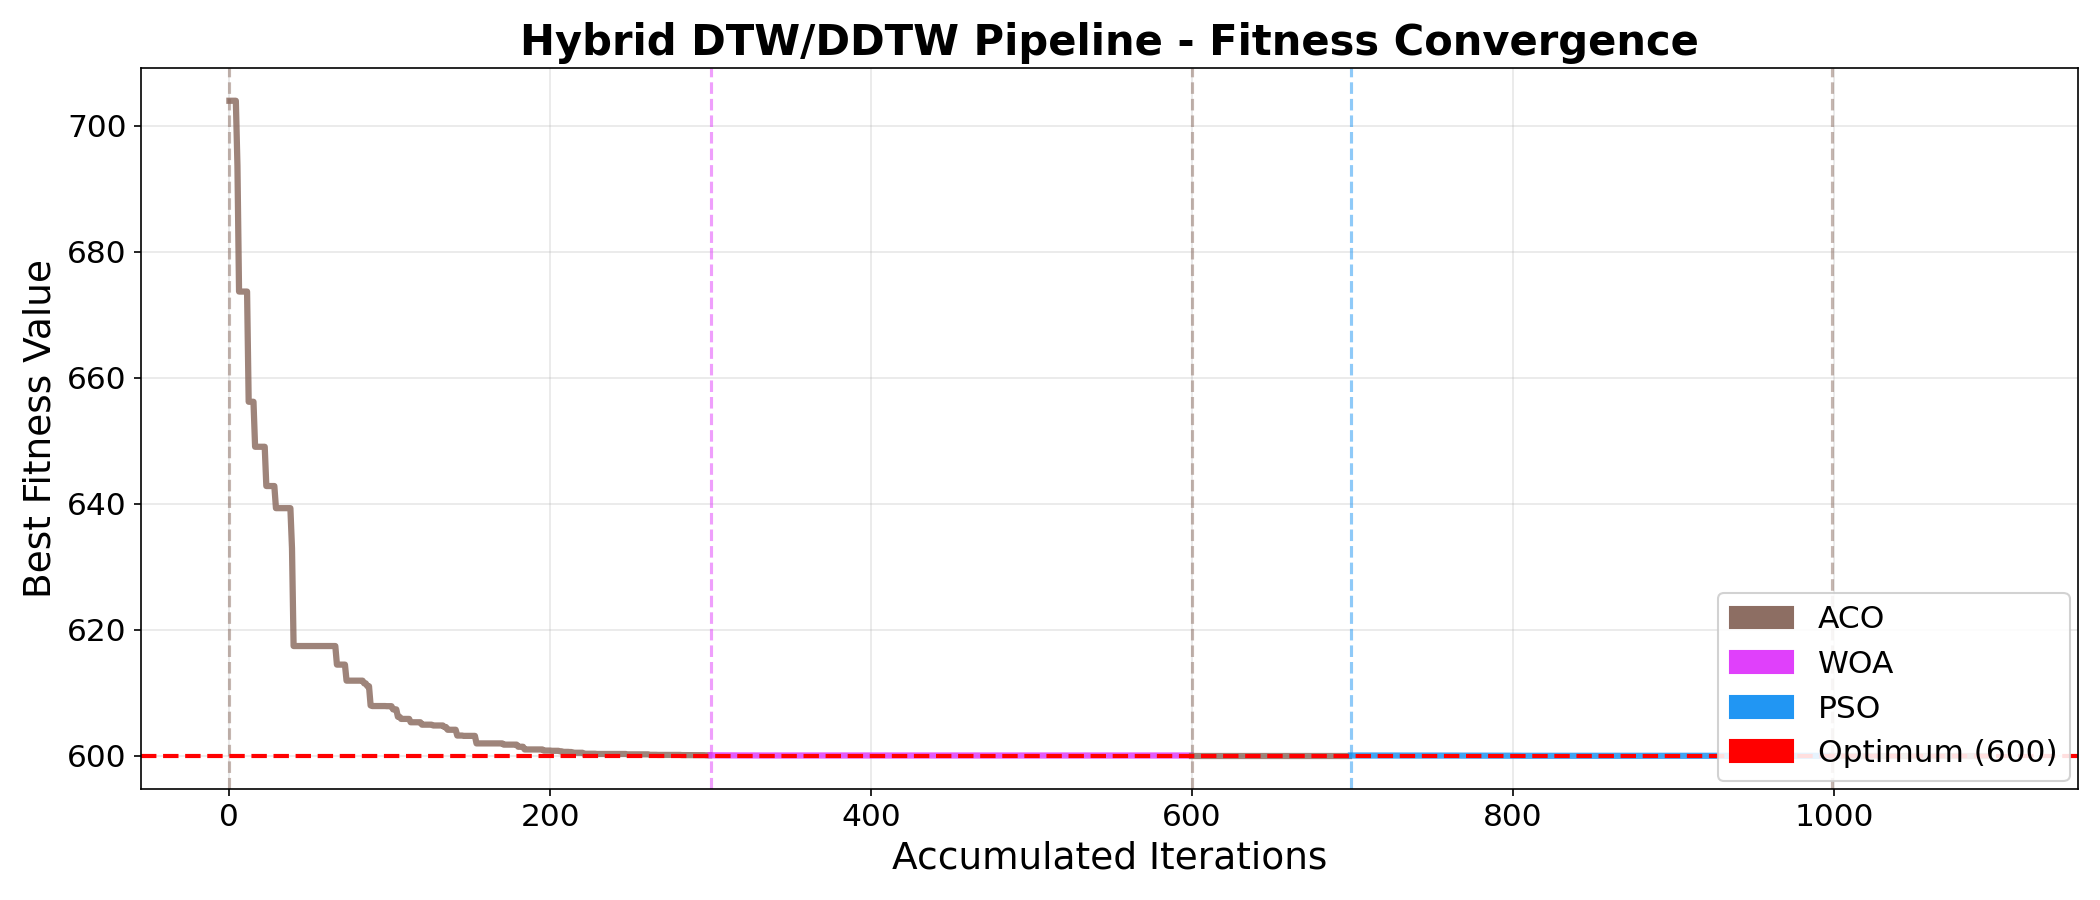
\includegraphics[width=0.7\linewidth]{imagenes_cec_mejores/cec_f3_dtw_convergencia.png}\hfill
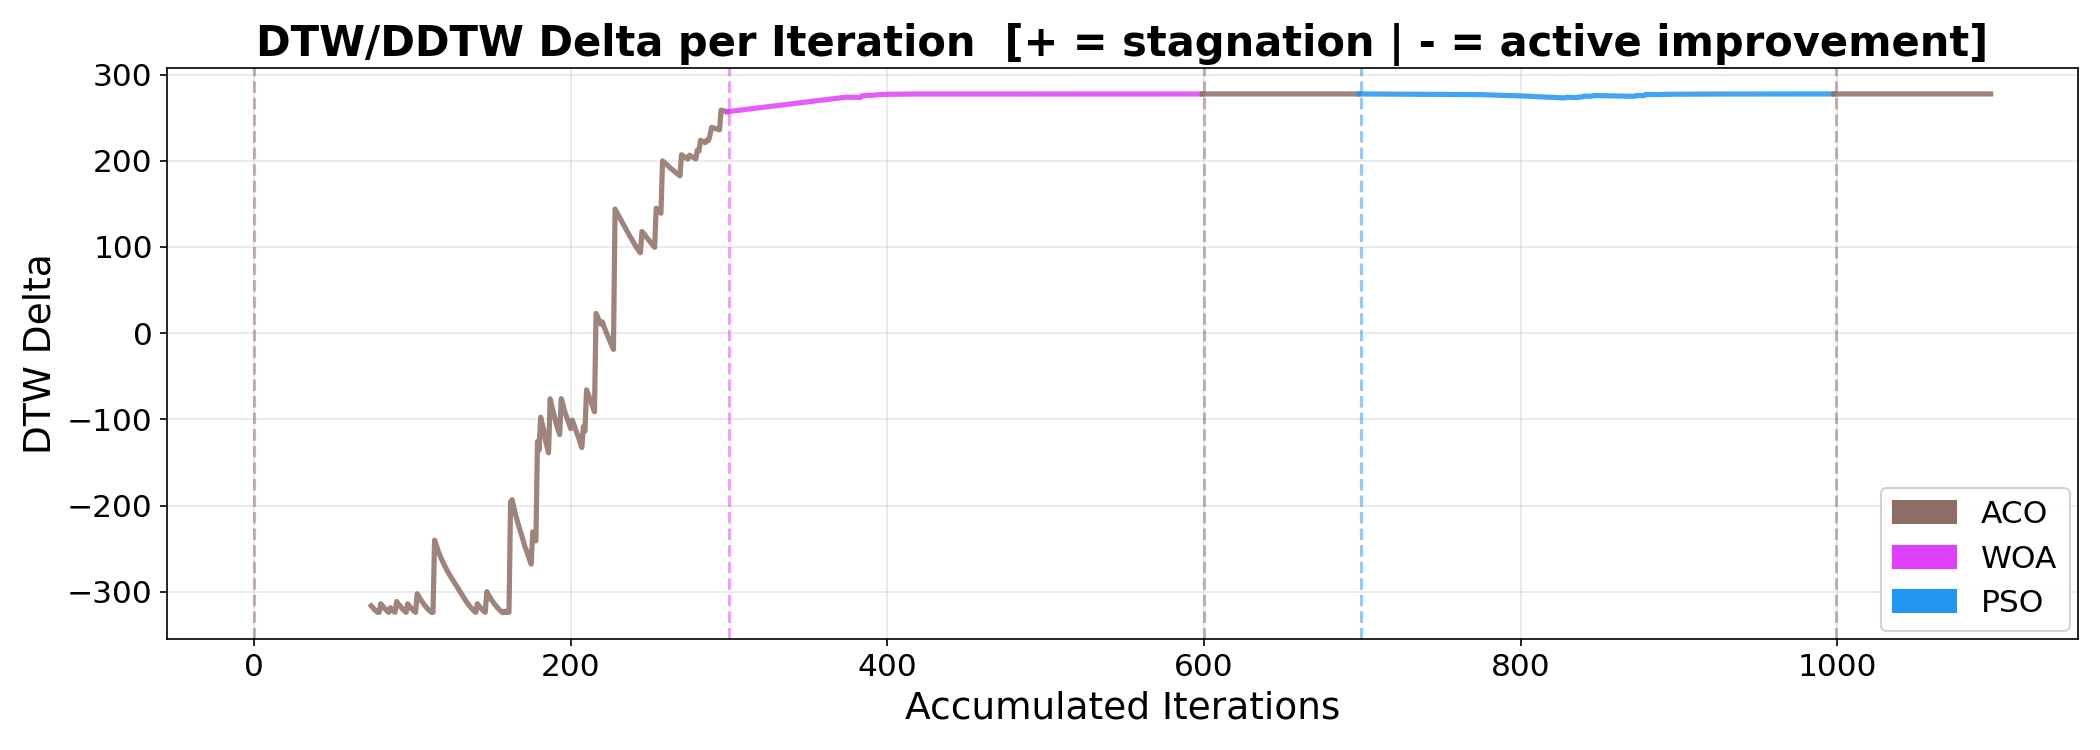
\includegraphics[width=0.7\linewidth]{imagenes_cec_mejores/cec_f3_dtw_dtw_delta.png}
\caption{Convergence trajectory (left) and $\Delta$ monitor (right) for
\texttt{F3} (Shifted Rotated Expanded Schaffers F7) under DTW, best run 14.}
\label{fig:cec-best-f3}
\end{figure}

\begin{figure}[H]
\centering
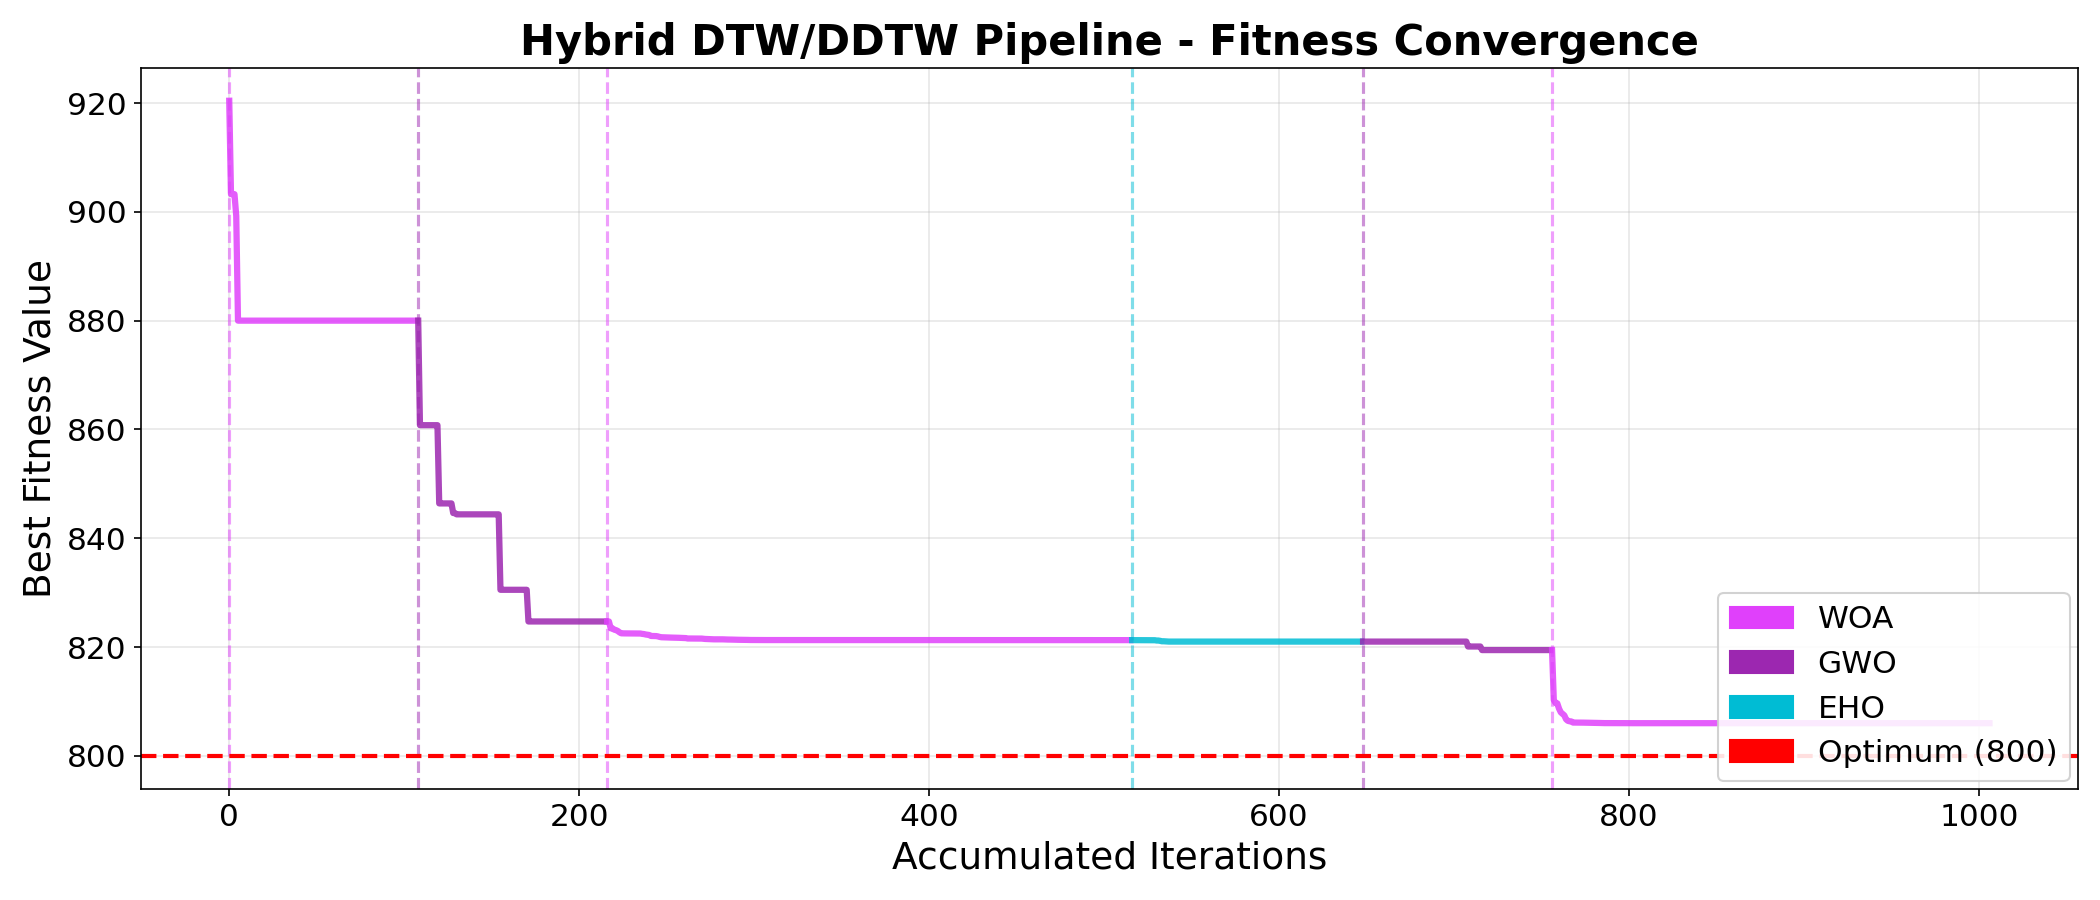
\includegraphics[width=0.7\linewidth]{imagenes_cec_mejores/cec_f4_ddtw_convergencia.png}\hfill
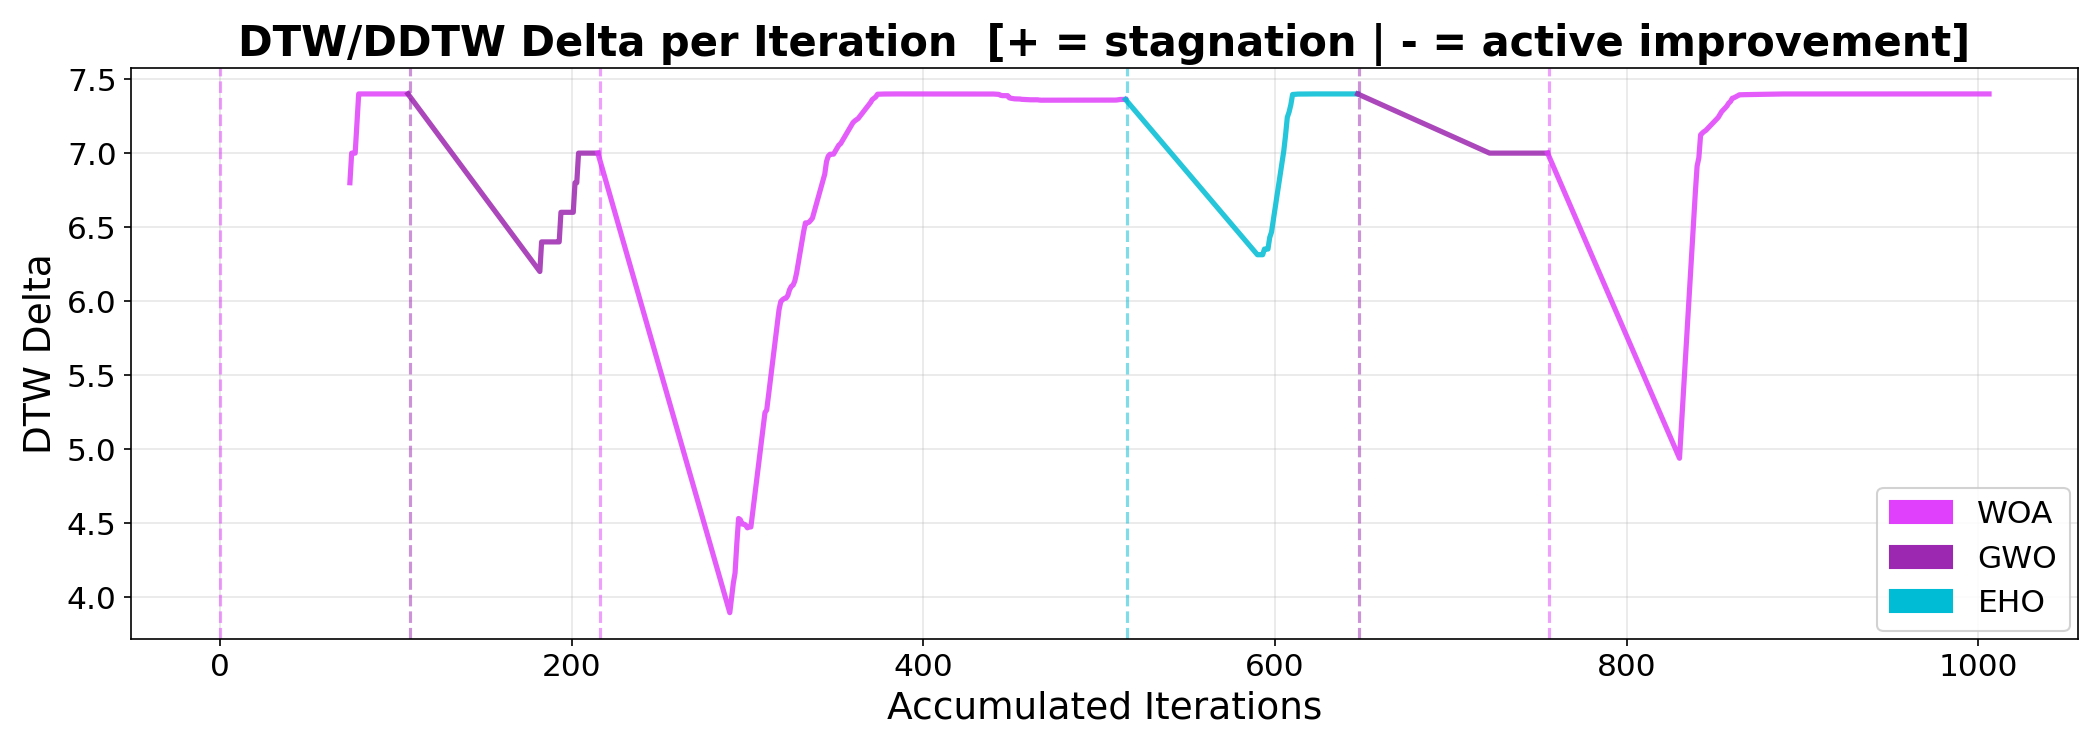
\includegraphics[width=0.7\linewidth]{imagenes_cec_mejores/cec_f4_ddtw_dtw_delta.png}
\caption{Convergence trajectory (left) and $\Delta$ monitor (right) for
\texttt{F4} (Shifted Rotated Non-Continuous Rastrigin) under DDTW, best run 30.}
\label{fig:cec-best-f4}
\end{figure}

\begin{figure}[H]
\centering
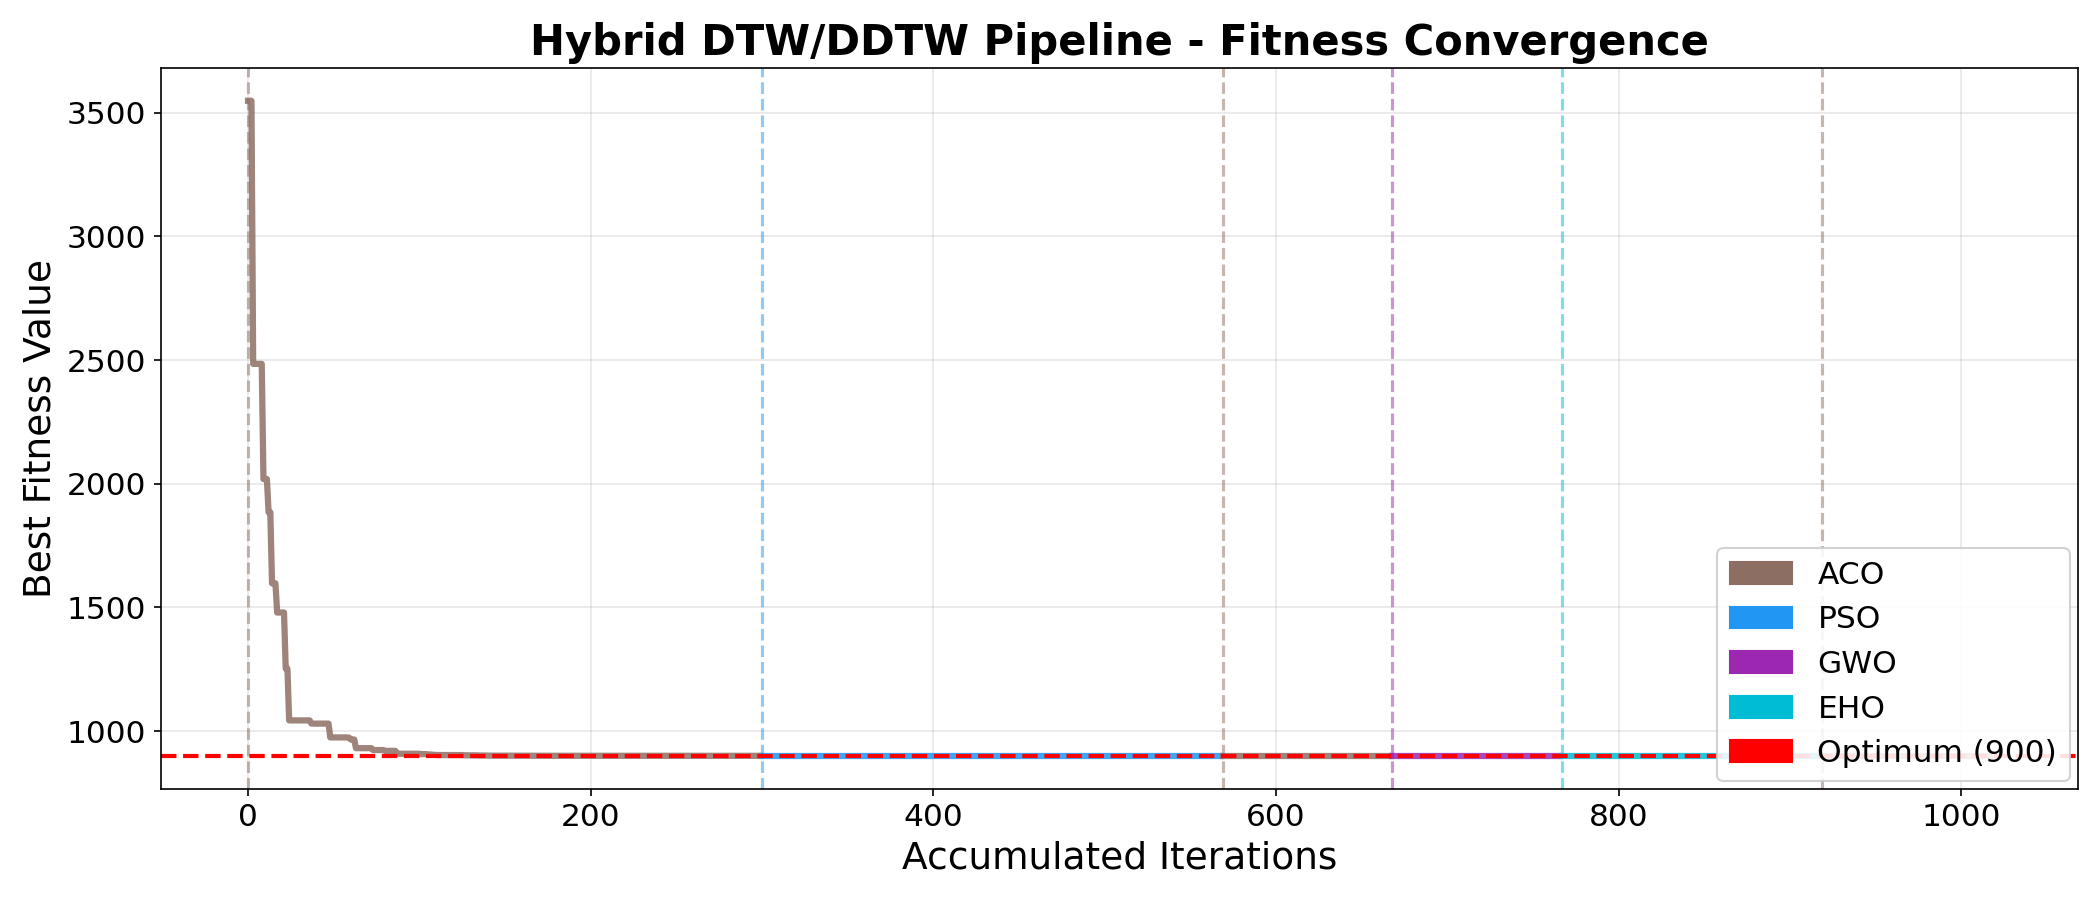
\includegraphics[width=0.7\linewidth]{imagenes_cec_mejores/cec_f5_dtw_convergencia.png}\hfill
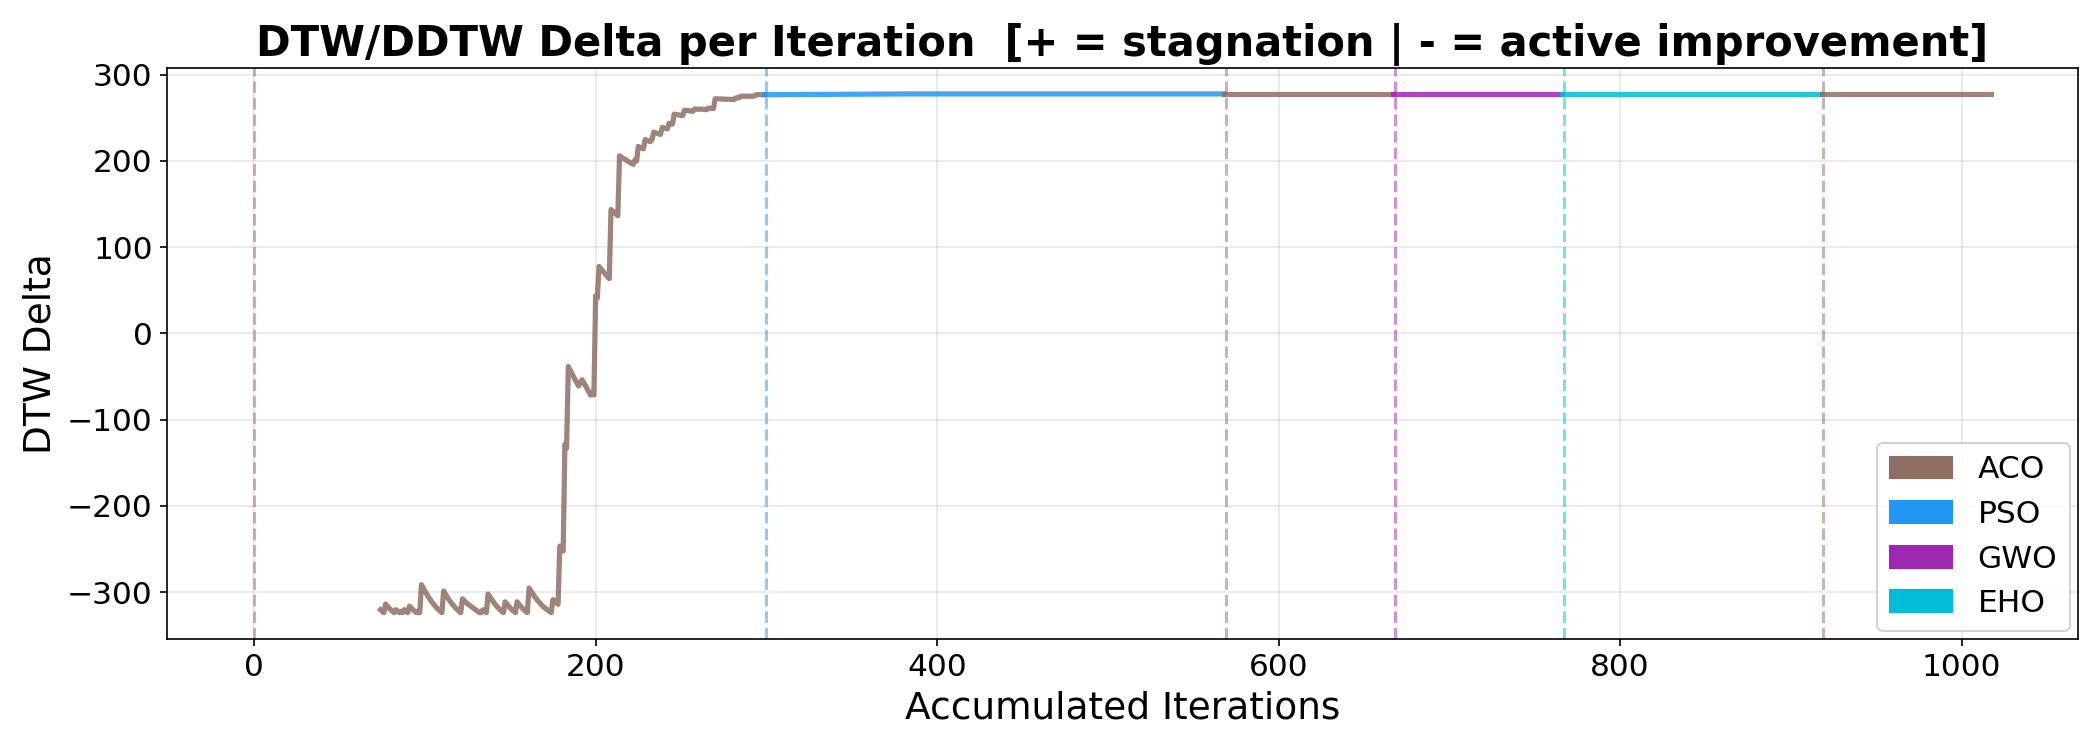
\includegraphics[width=0.7\linewidth]{imagenes_cec_mejores/cec_f5_dtw_dtw_delta.png}
\caption{Convergence trajectory (left) and $\Delta$ monitor (right) for
\texttt{F5} (Shifted Rotated Levy) under DTW, best run 11.}
\label{fig:cec-best-f5}
\end{figure}

\begin{figure}[H]
\centering
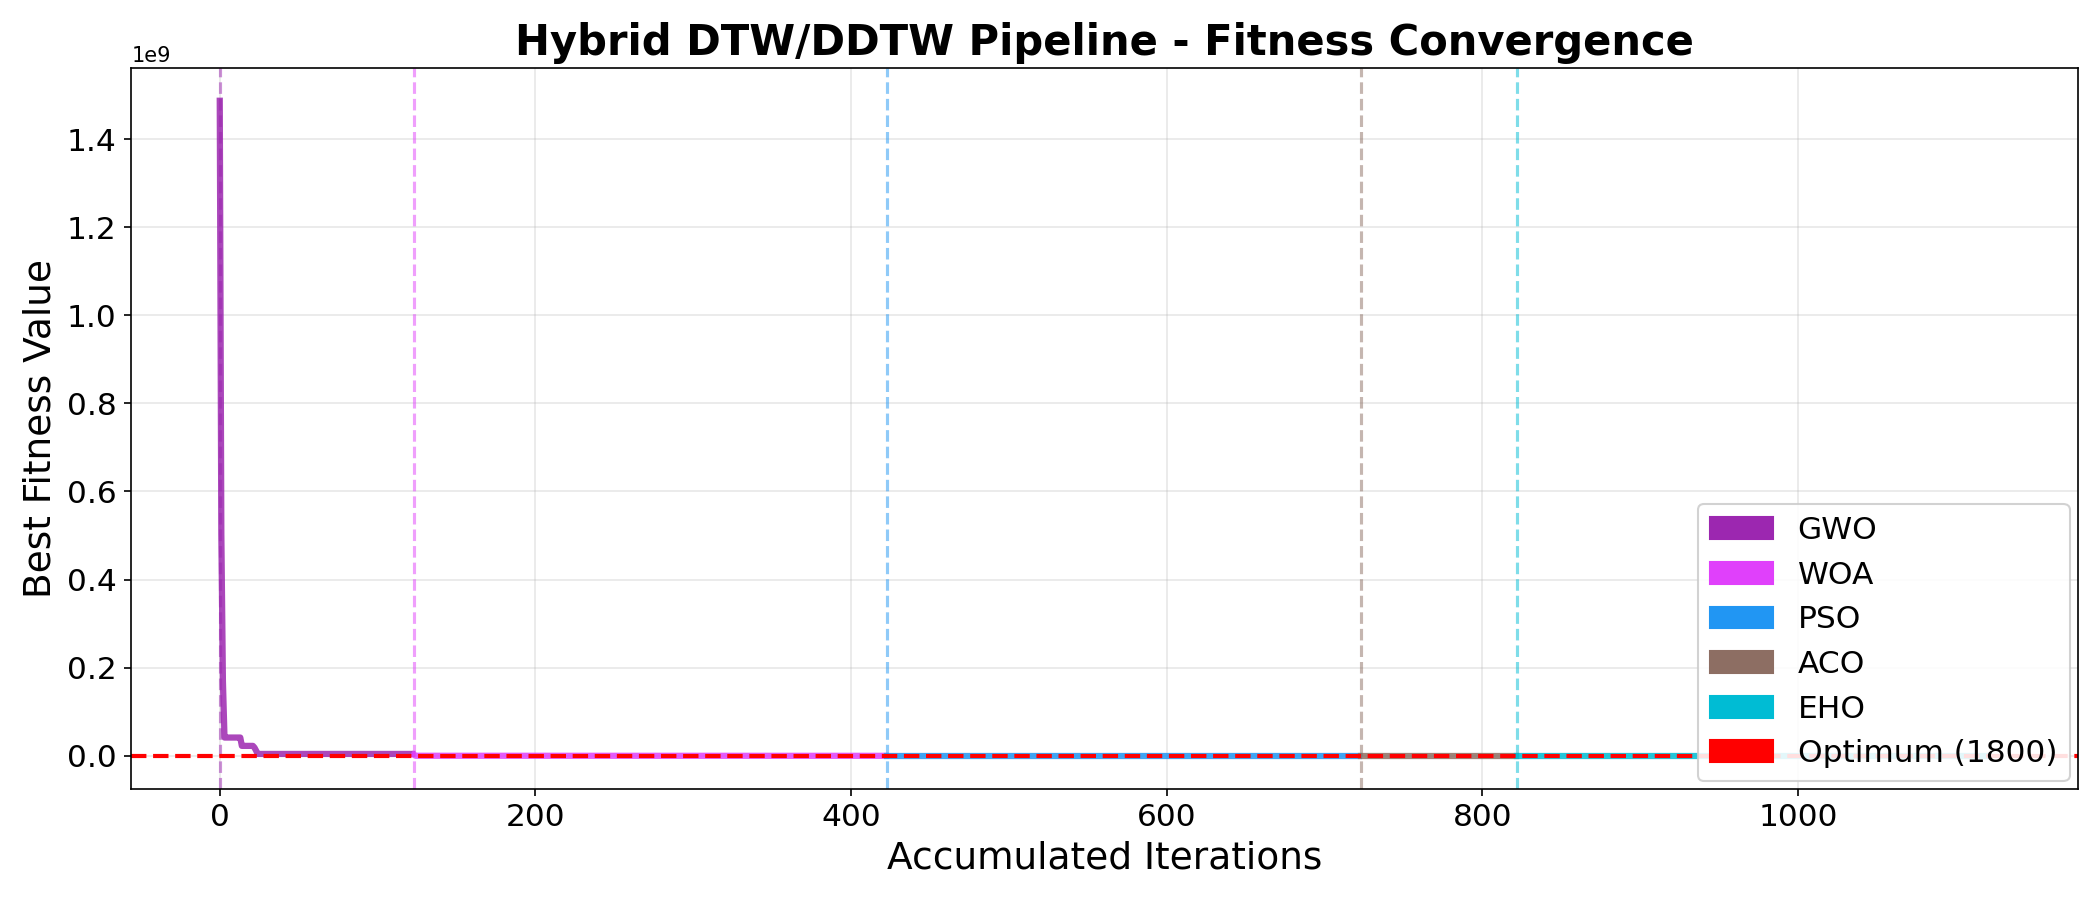
\includegraphics[width=0.7\linewidth]{imagenes_cec_mejores/cec_f6_dtw_convergencia.png}\hfill
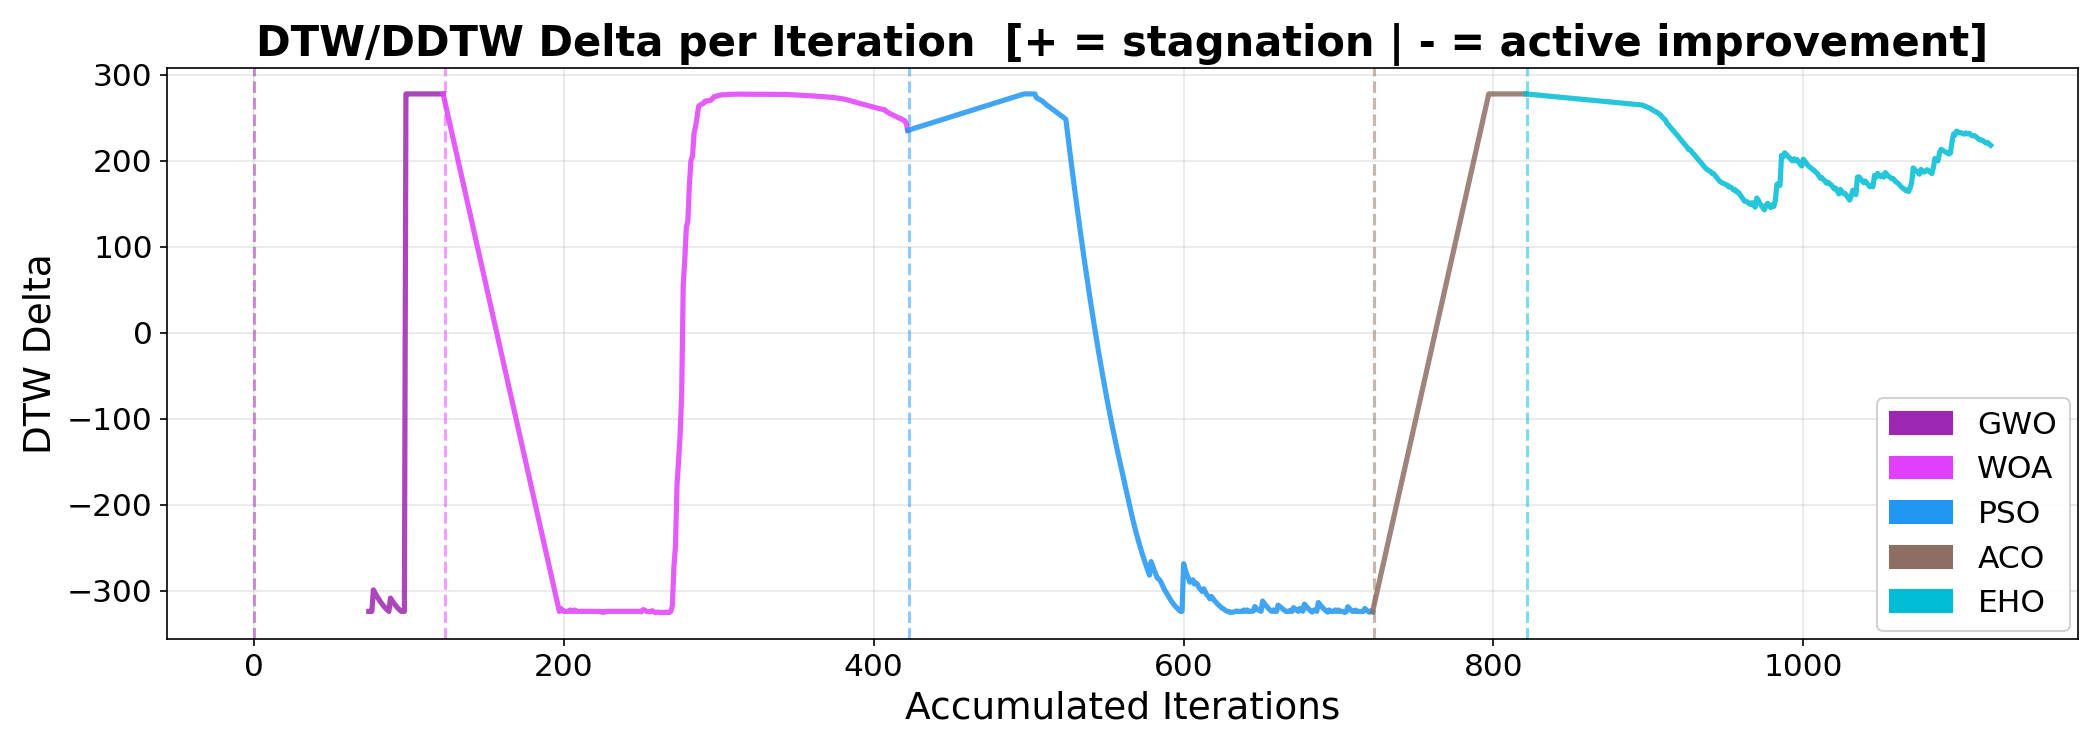
\includegraphics[width=0.7\linewidth]{imagenes_cec_mejores/cec_f6_dtw_dtw_delta.png}
\caption{Convergence trajectory (left) and $\Delta$ monitor (right) for
\texttt{F6} (Hybrid Function 1) under DTW, best run 02.}
\label{fig:cec-best-f6}
\end{figure}

\begin{figure}[H]
\centering
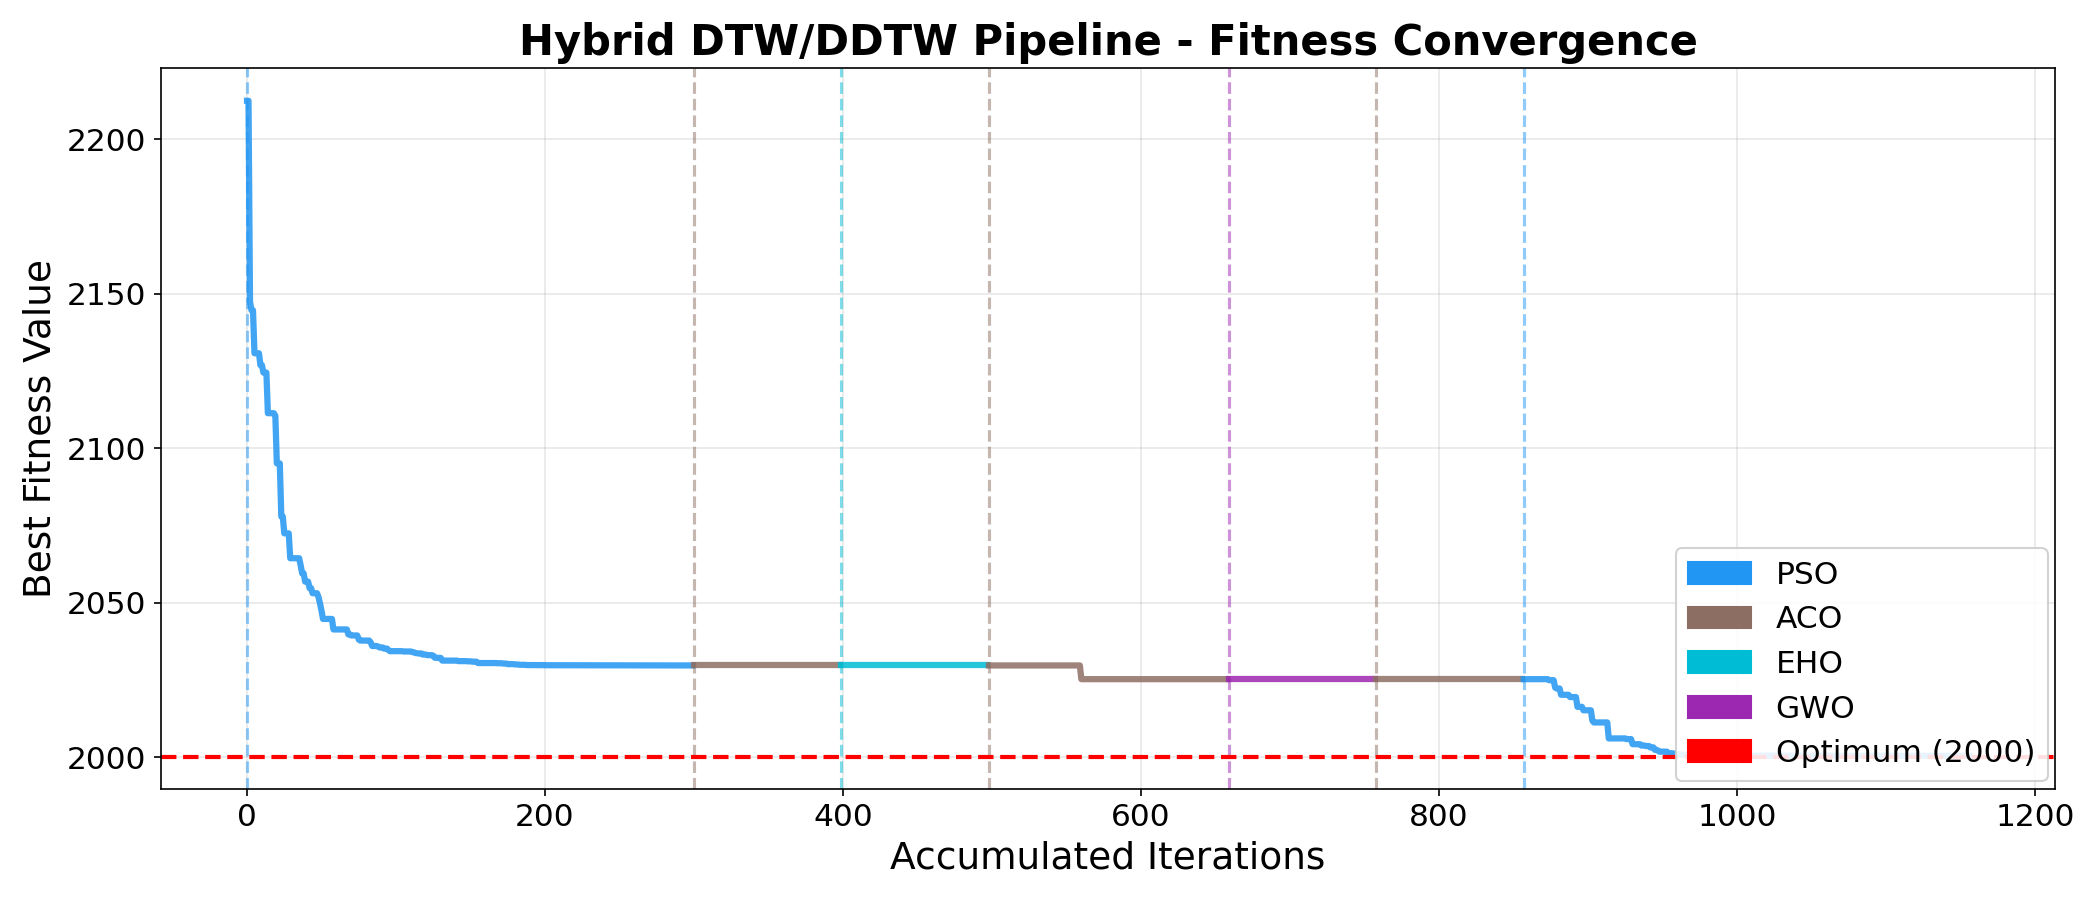
\includegraphics[width=0.7\linewidth]{imagenes_cec_mejores/cec_f7_dtw_convergencia.png}\hfill
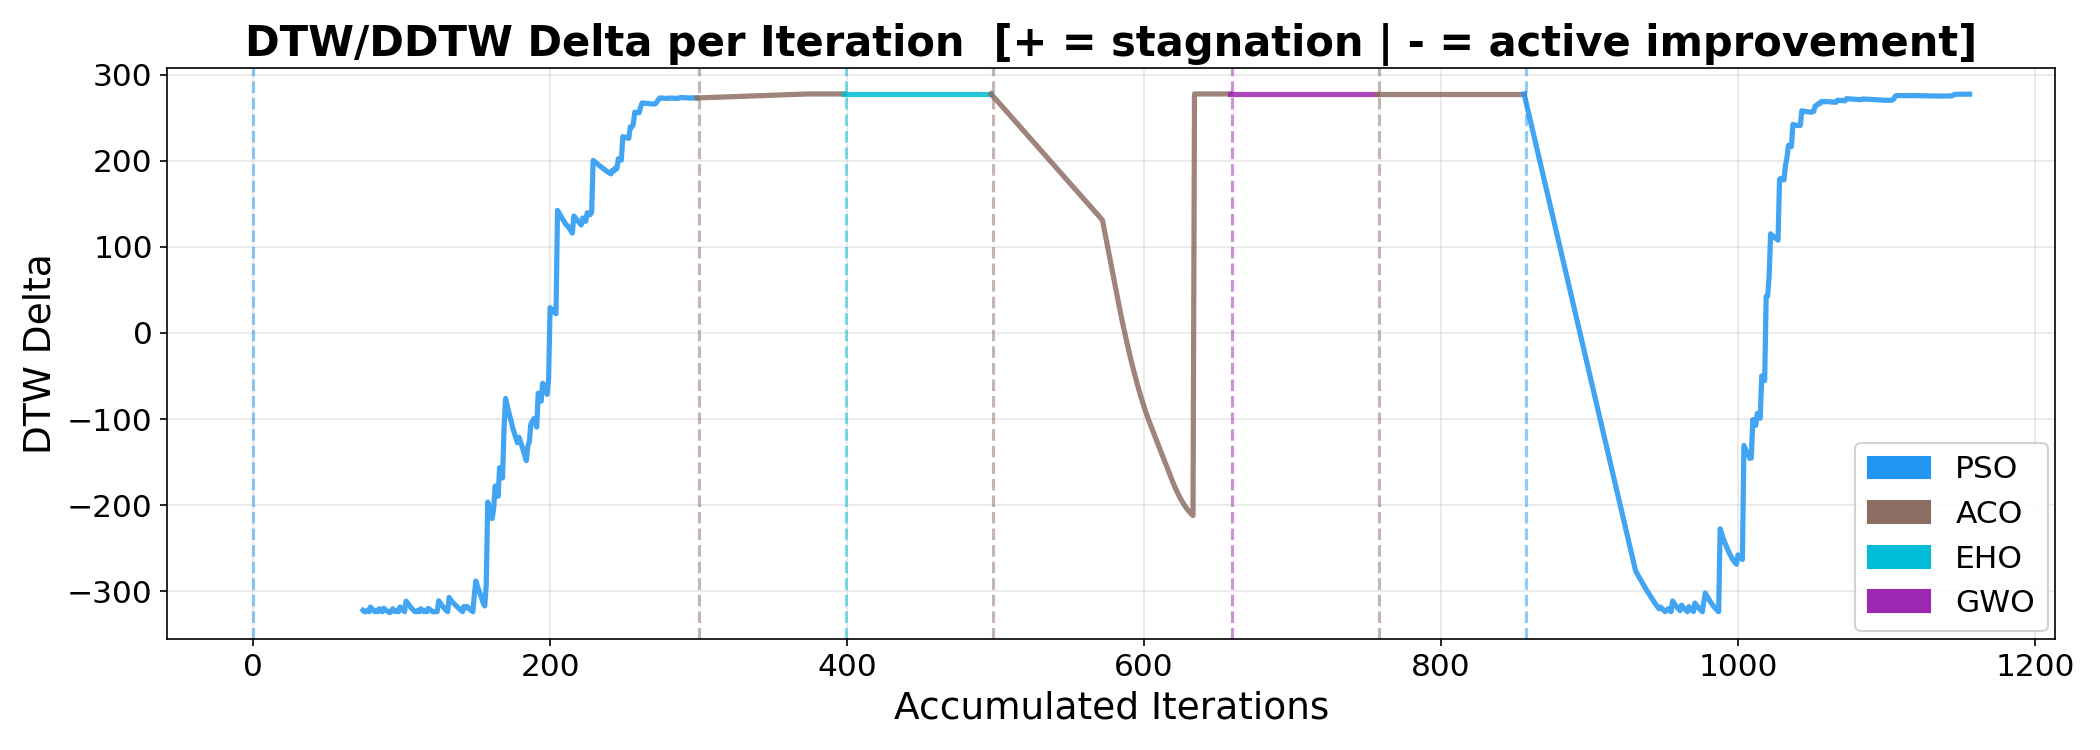
\includegraphics[width=0.7\linewidth]{imagenes_cec_mejores/cec_f7_dtw_dtw_delta.png}
\caption{Convergence trajectory (left) and $\Delta$ monitor (right) for
\texttt{F7} (Hybrid Function 2) under DTW, best run 12.}
\label{fig:cec-best-f7}
\end{figure}

\begin{figure}[H]
\centering
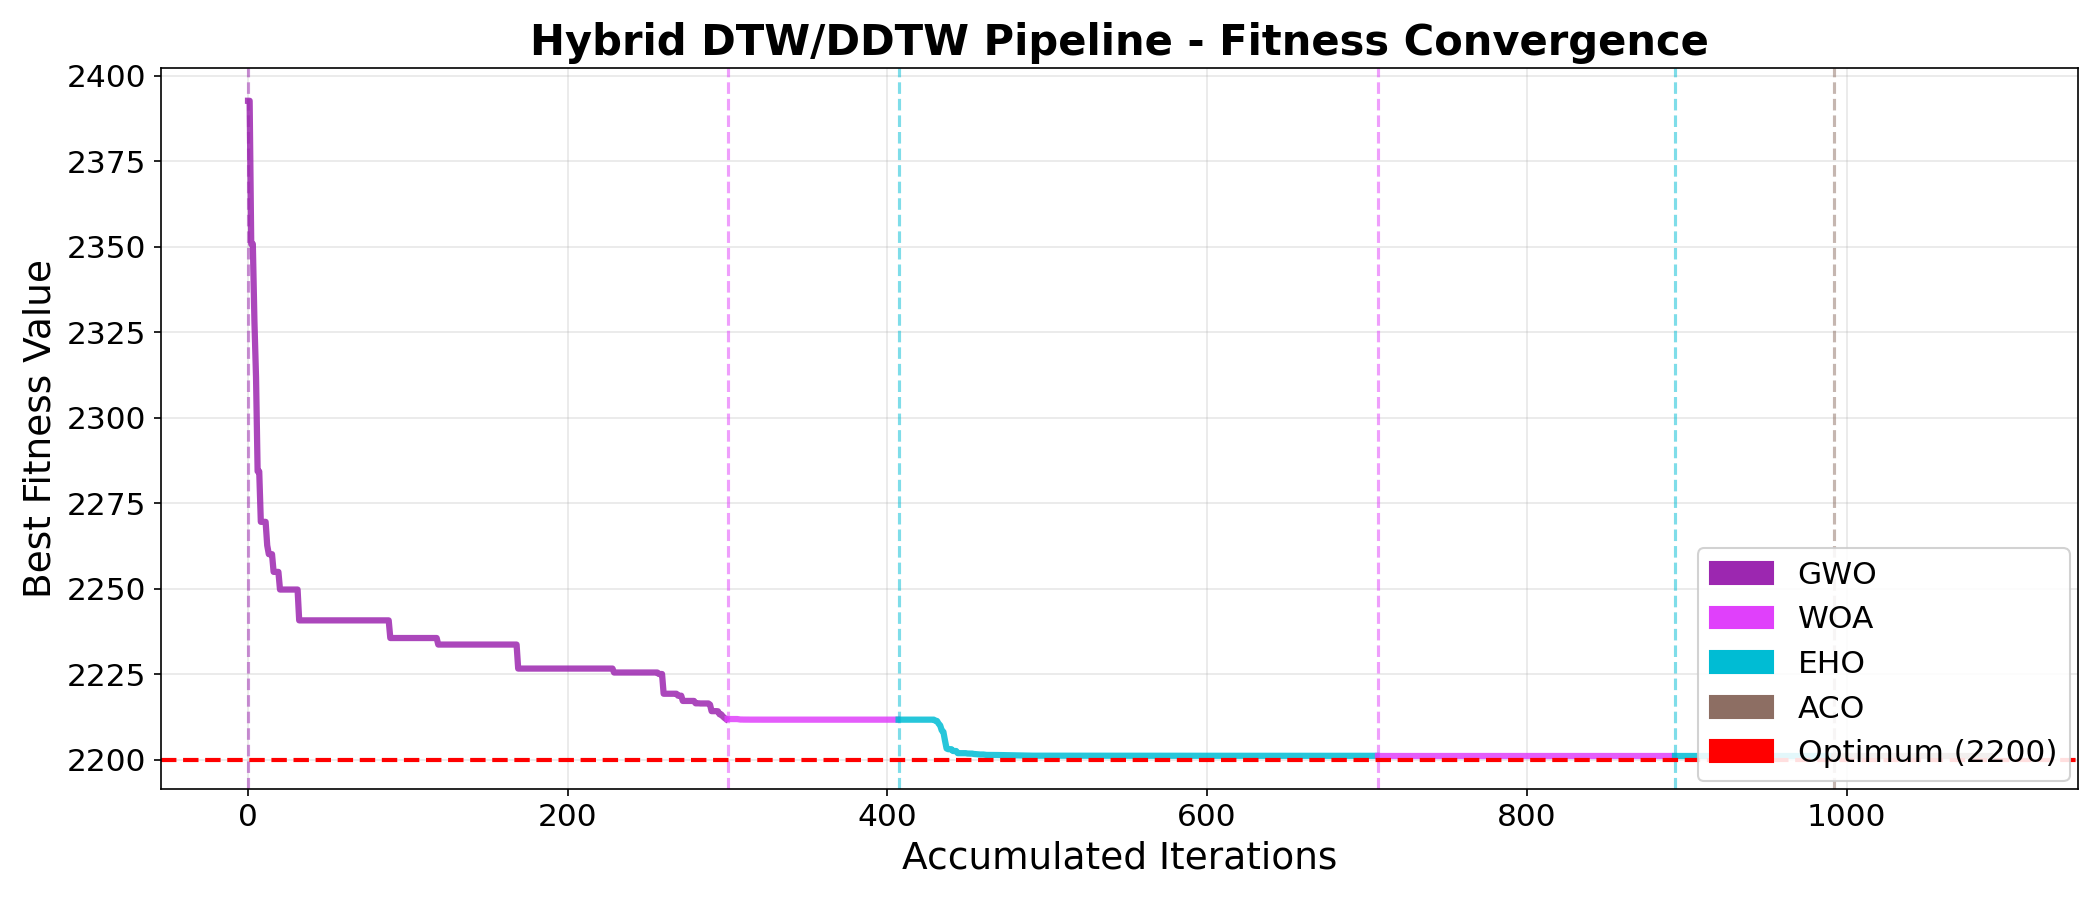
\includegraphics[width=0.7\linewidth]{imagenes_cec_mejores/cec_f8_dtw_convergencia.png}\hfill
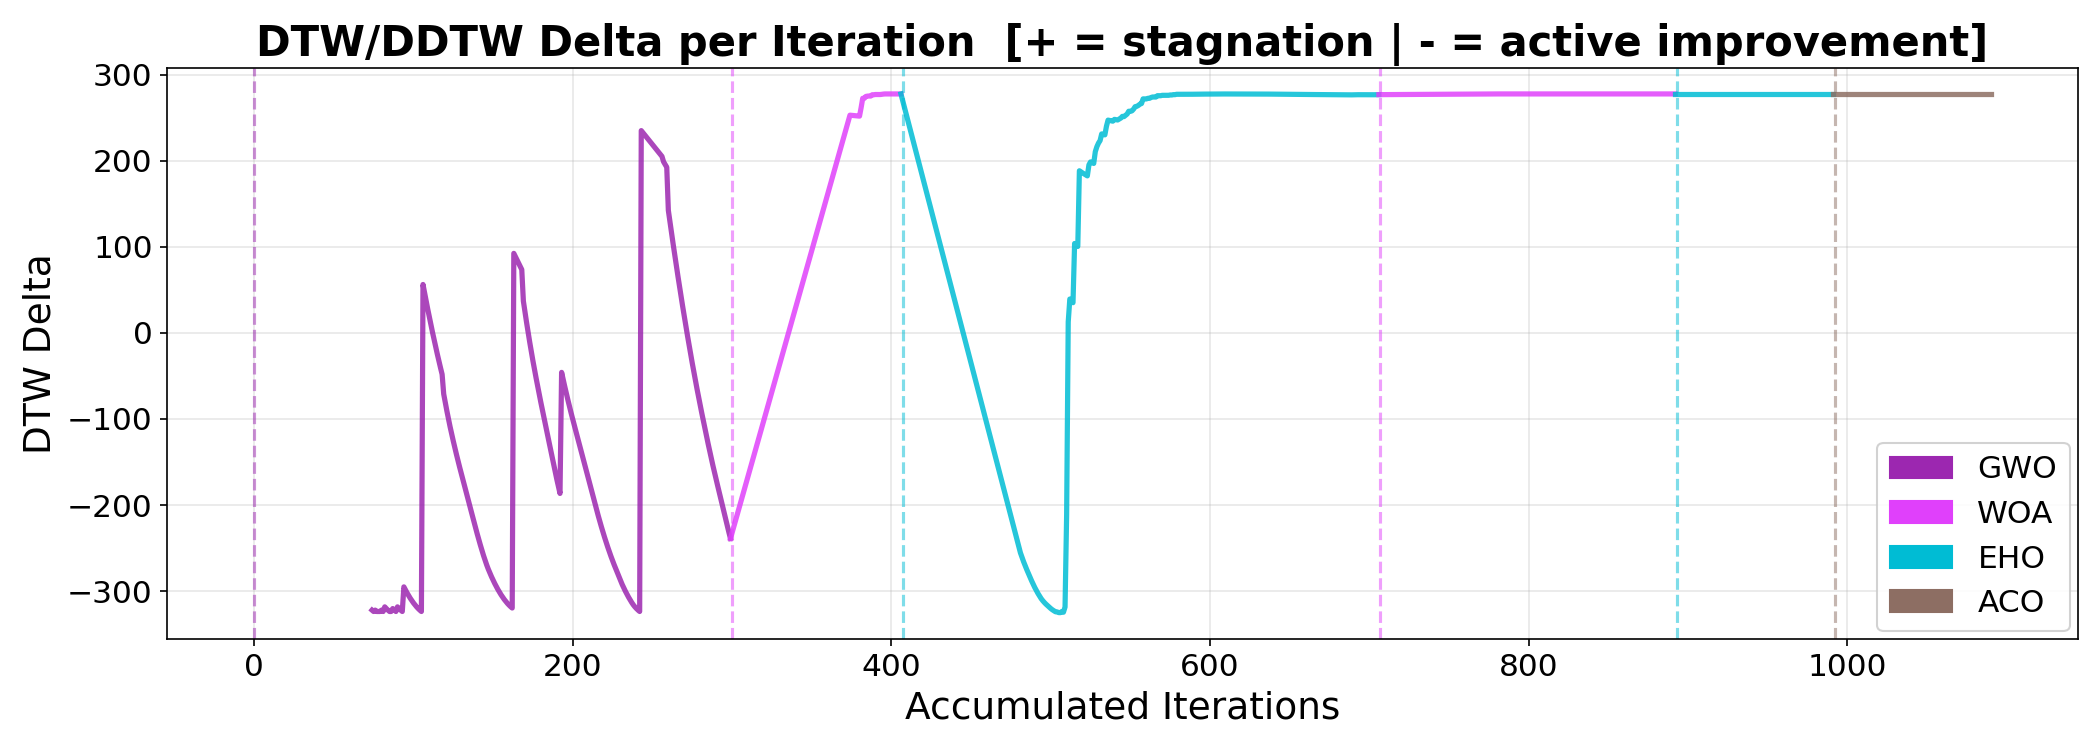
\includegraphics[width=0.7\linewidth]{imagenes_cec_mejores/cec_f8_dtw_dtw_delta.png}
\caption{Convergence trajectory (left) and $\Delta$ monitor (right) for
\texttt{F8} (Hybrid Function 3) under DTW, best run 26.}
\label{fig:cec-best-f8}
\end{figure}

\begin{figure}[H]
\centering
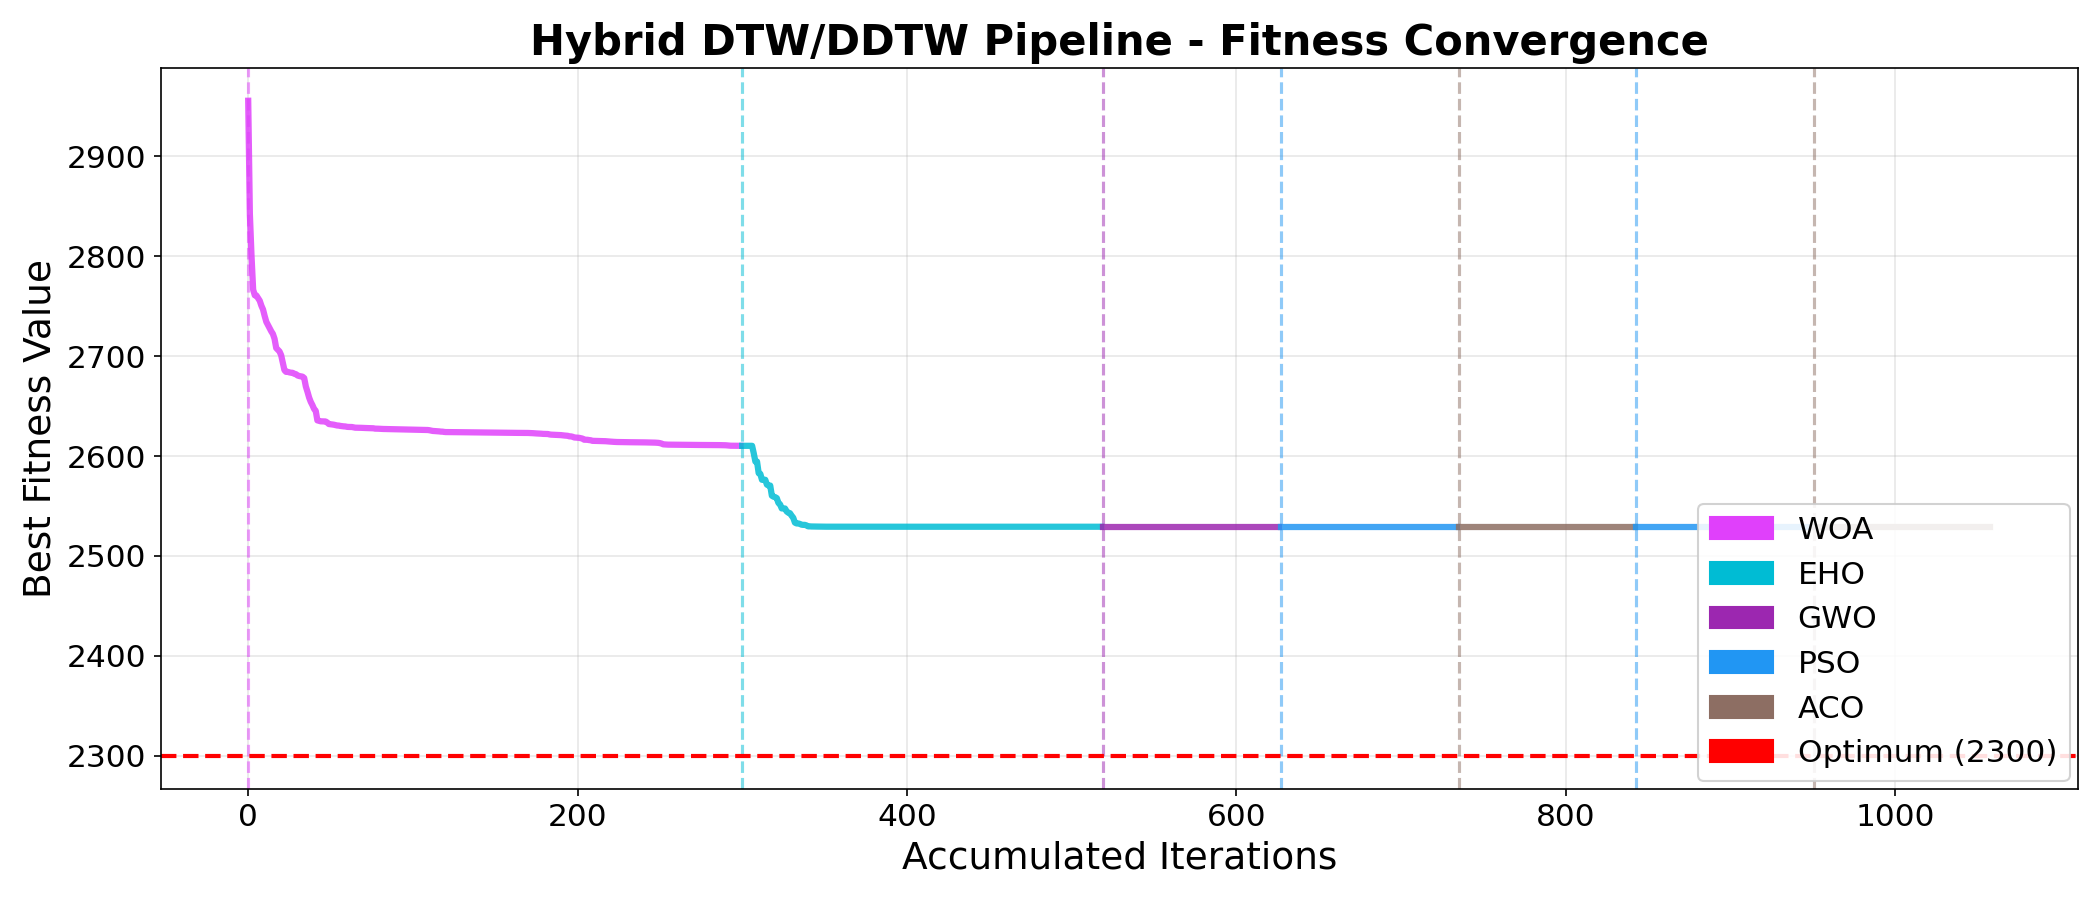
\includegraphics[width=0.7\linewidth]{imagenes_cec_mejores/cec_f9_ddtw_convergencia.png}\hfill
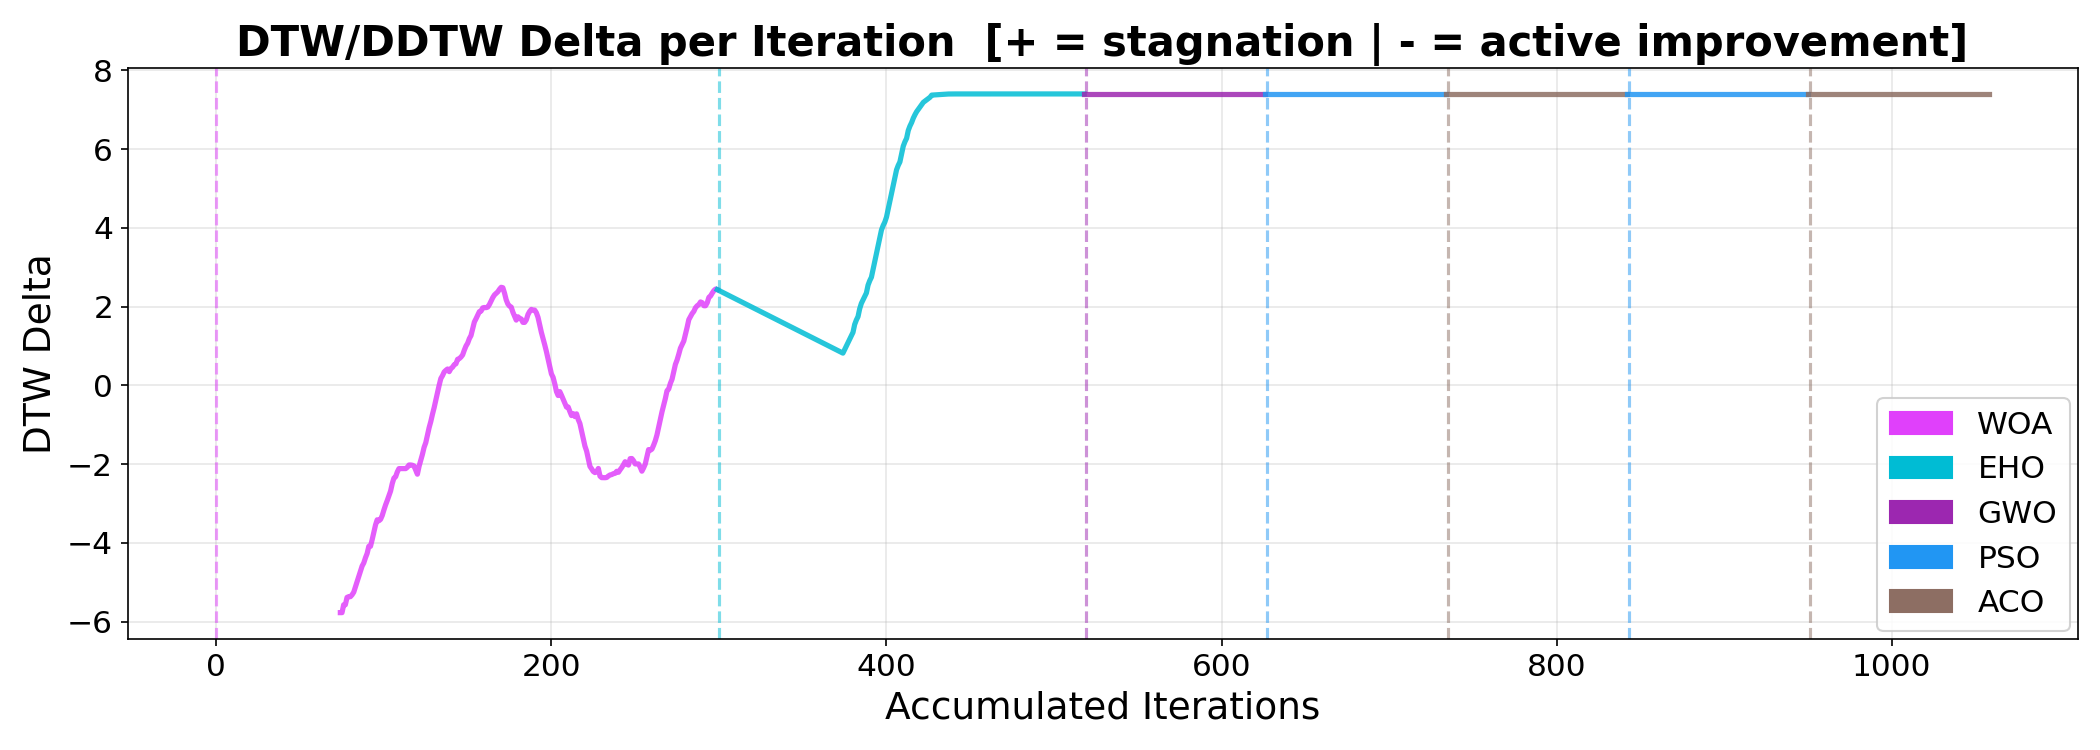
\includegraphics[width=0.7\linewidth]{imagenes_cec_mejores/cec_f9_ddtw_dtw_delta.png}
\caption{Convergence trajectory (left) and $\Delta$ monitor (right) for
\texttt{F9} (Composition Function 1) under DDTW, best run 01.}
\label{fig:cec-best-f9}
\end{figure}

\begin{figure}[H]
\centering
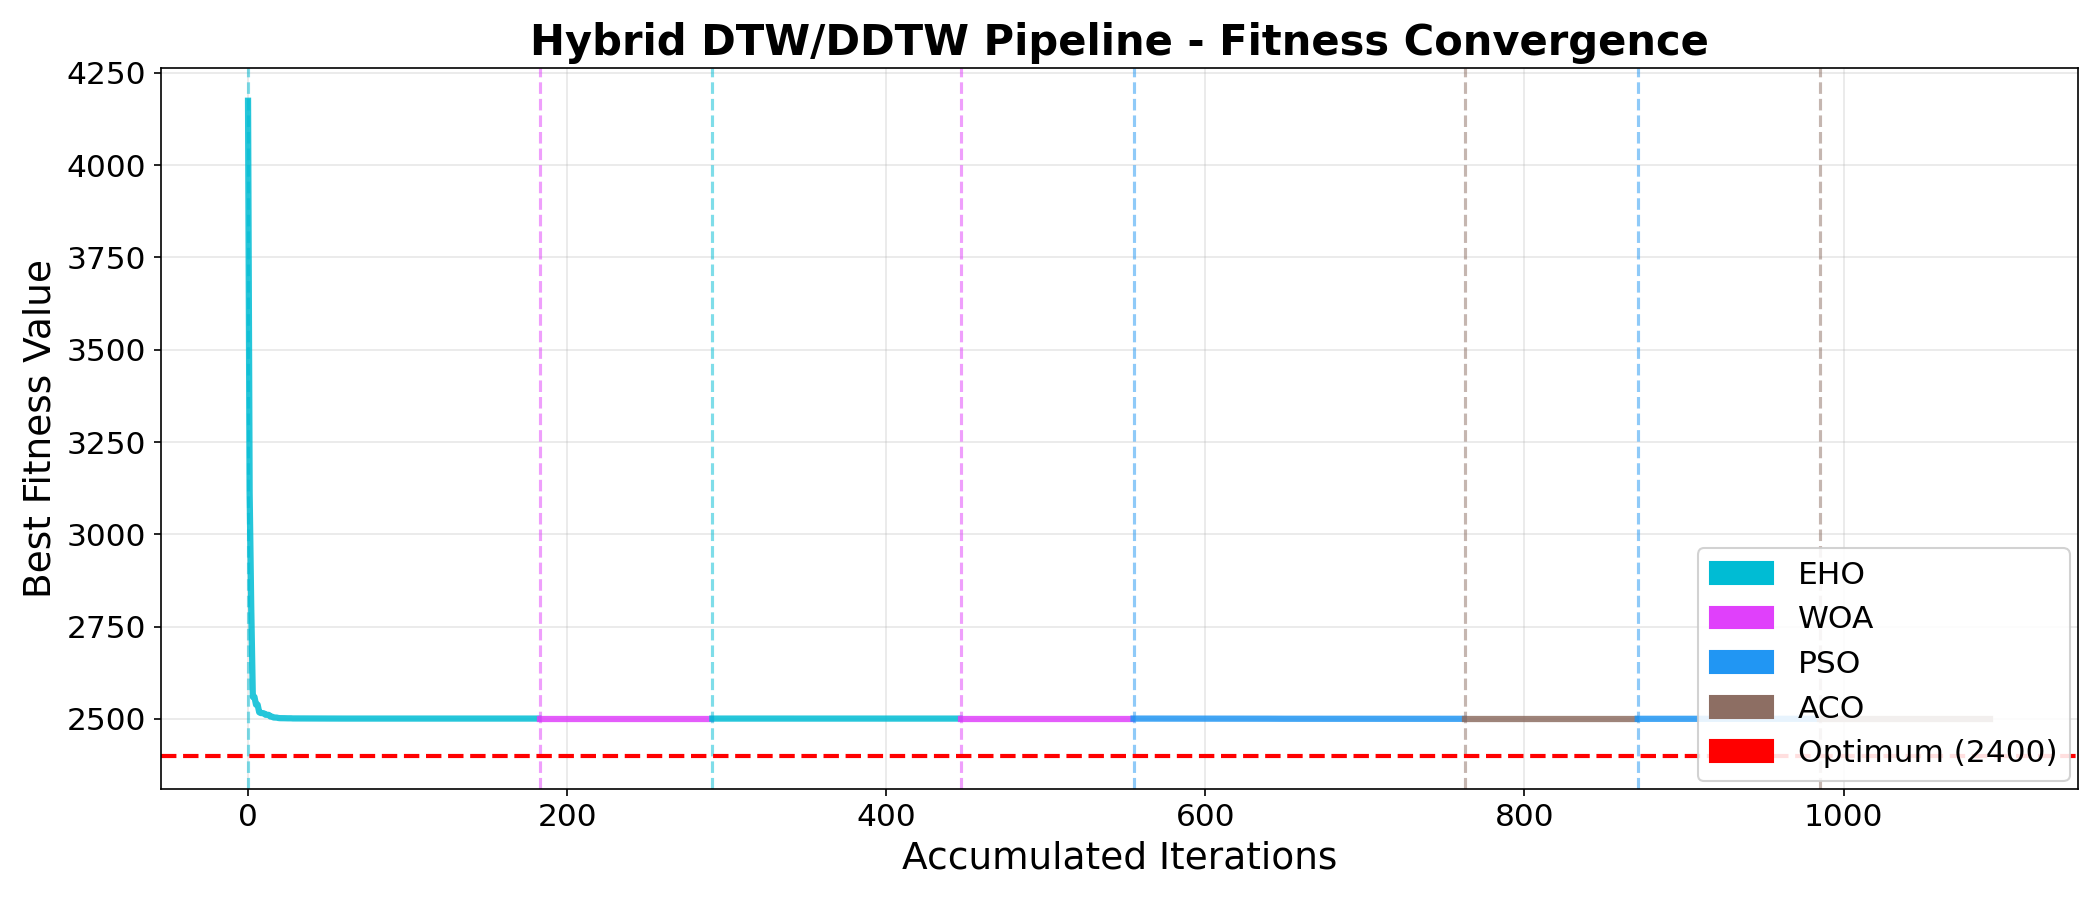
\includegraphics[width=0.7\linewidth]{imagenes_cec_mejores/cec_f10_ddtw_convergencia.png}\hfill
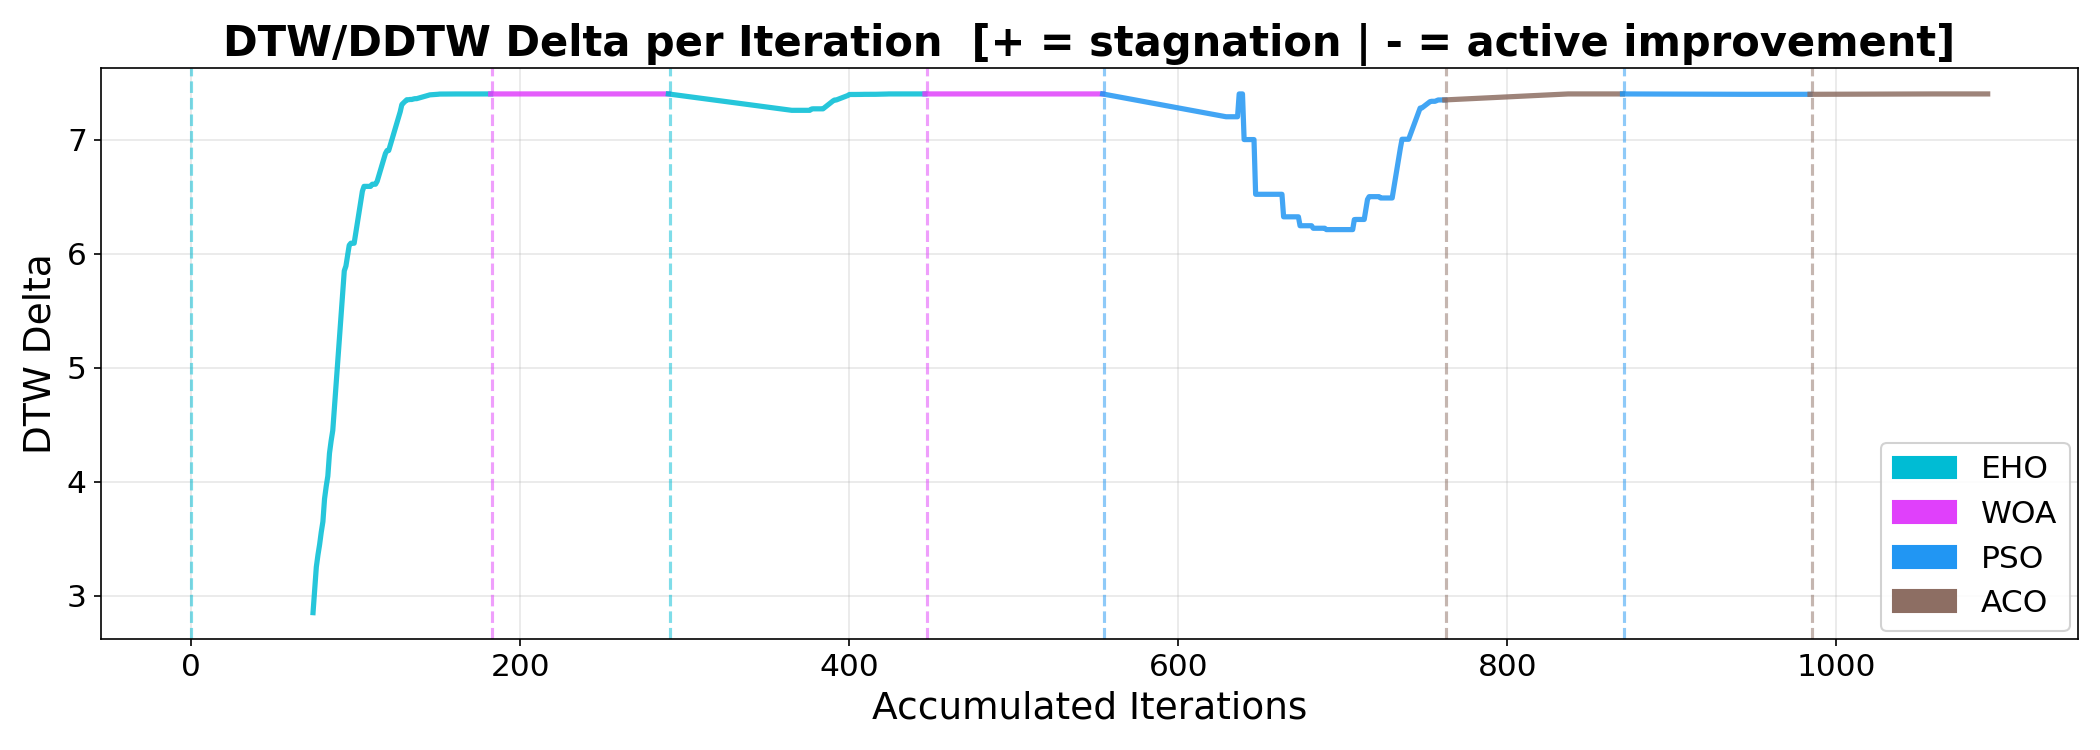
\includegraphics[width=0.7\linewidth]{imagenes_cec_mejores/cec_f10_ddtw_dtw_delta.png}
\caption{Convergence trajectory (left) and $\Delta$ monitor (right) for
\texttt{F10} (Composition Function 2) under DDTW, best run 29.}
\label{fig:cec-best-f10}
\end{figure}

\begin{figure}[H]
\centering
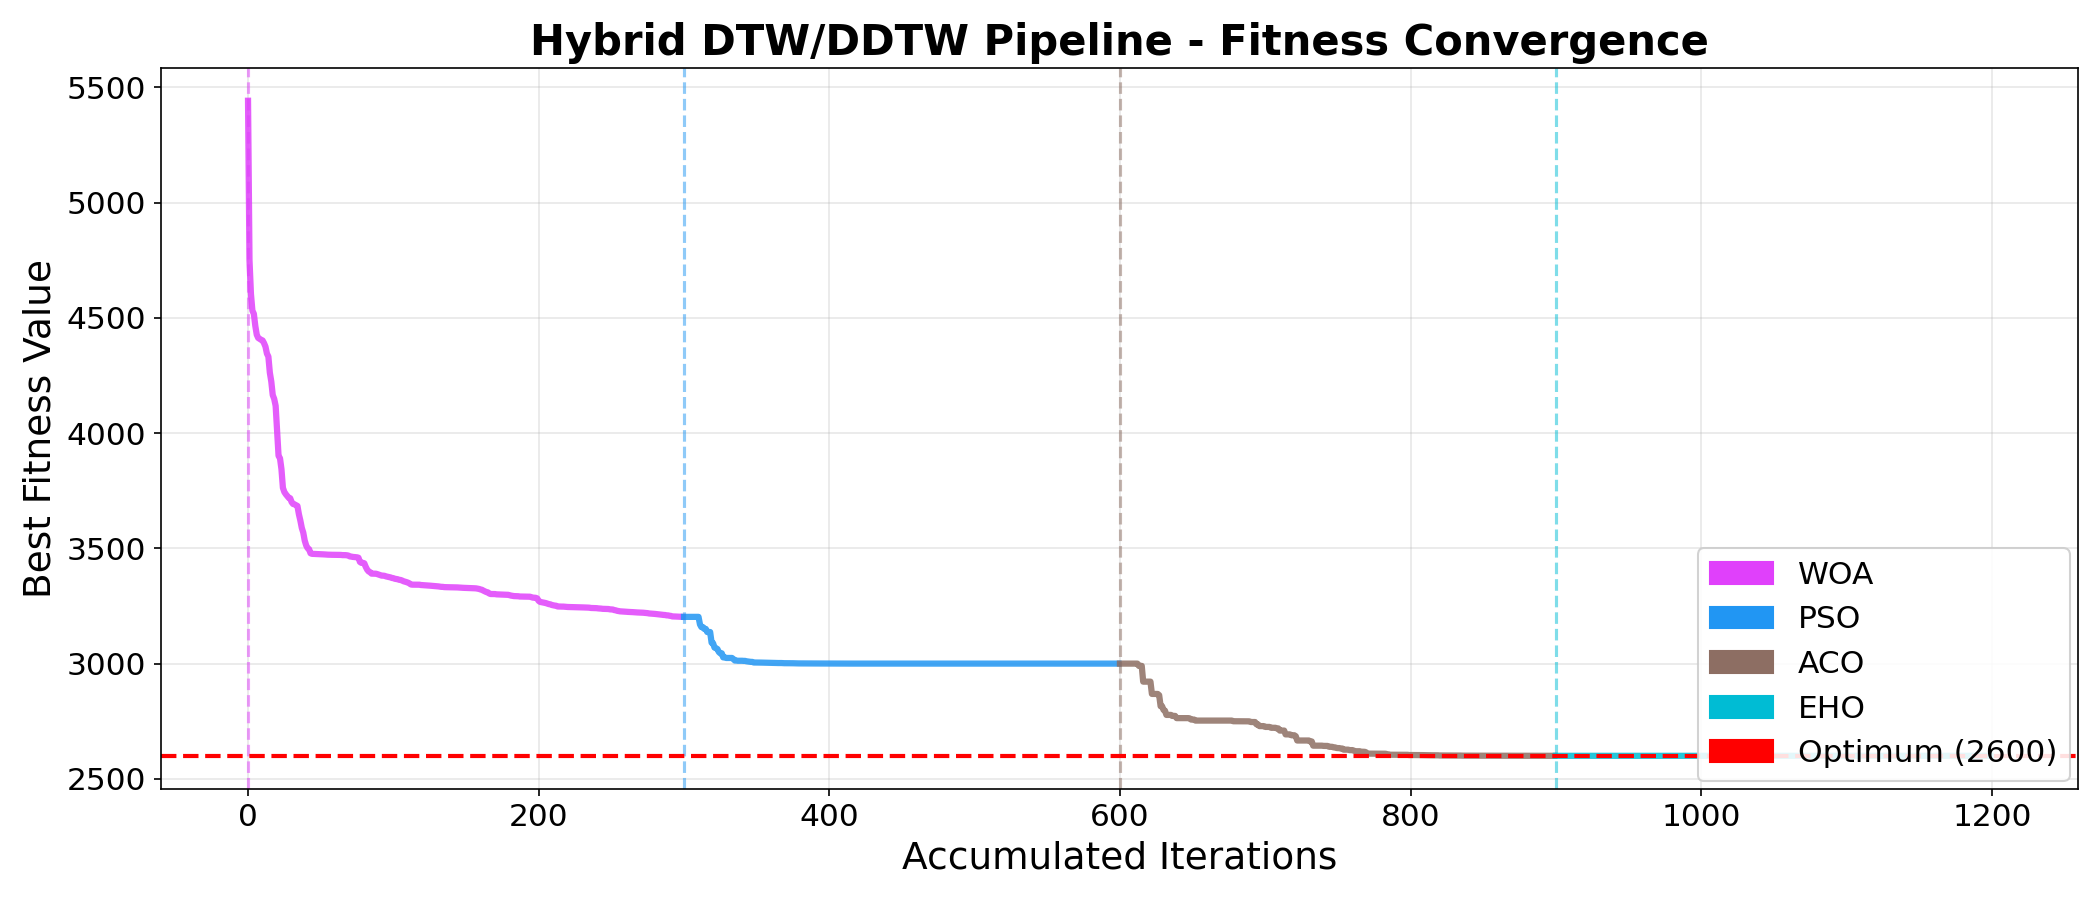
\includegraphics[width=0.7\linewidth]{imagenes_cec_mejores/cec_f11_dtw_convergencia.png}\hfill
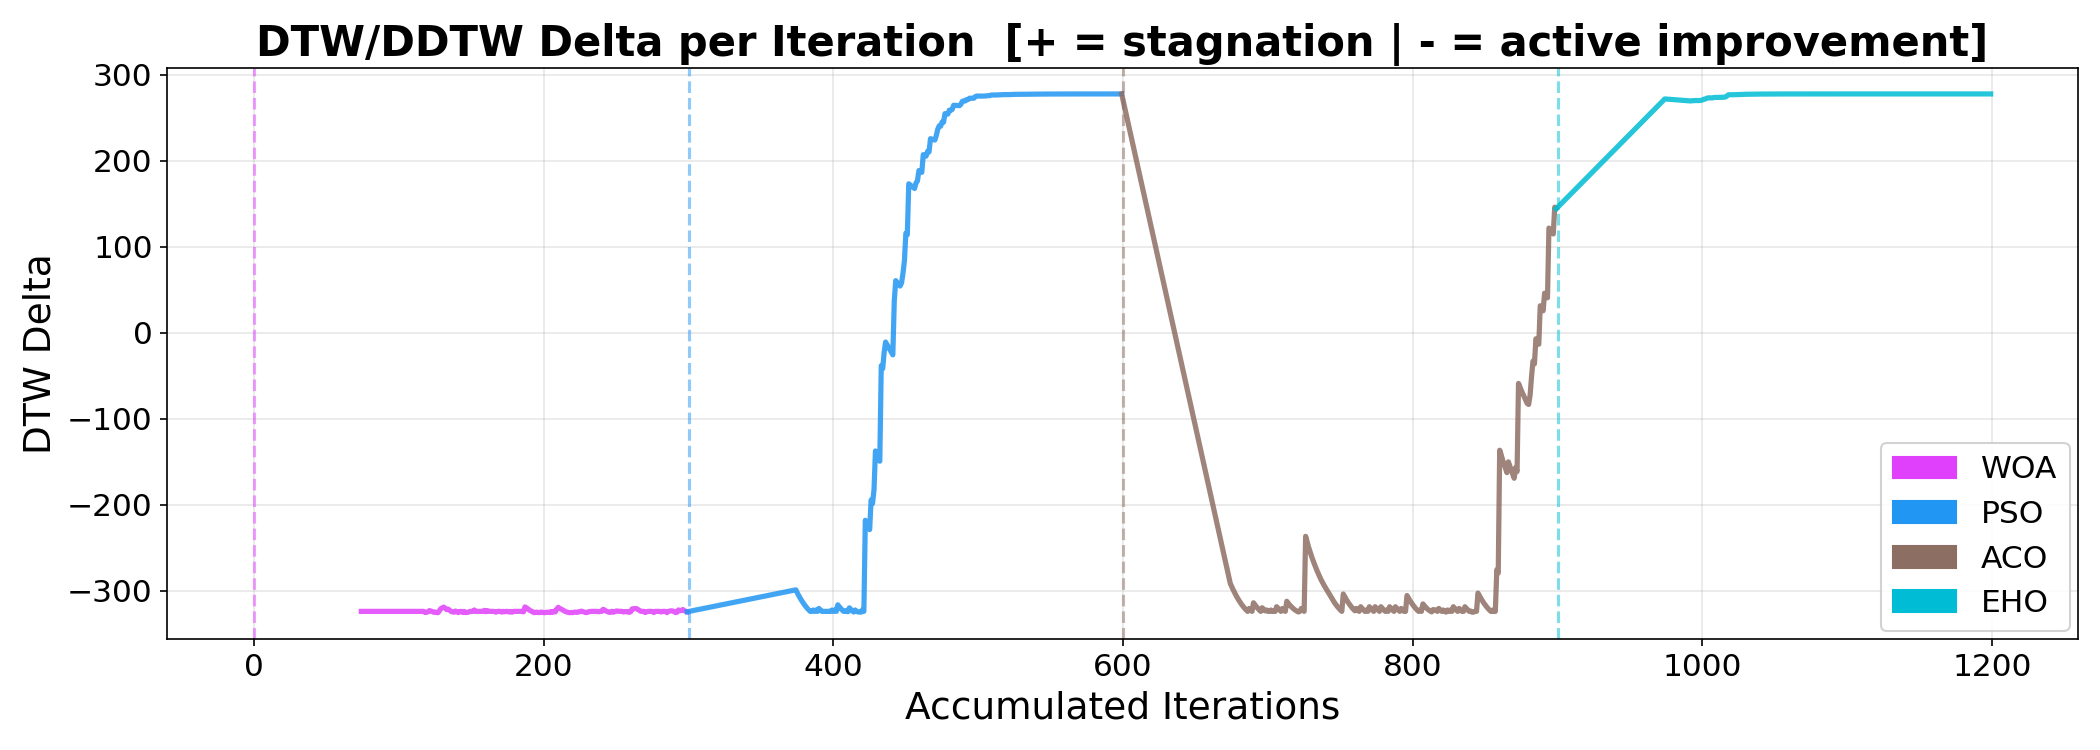
\includegraphics[width=0.7\linewidth]{imagenes_cec_mejores/cec_f11_dtw_dtw_delta.png}
\caption{Convergence trajectory (left) and $\Delta$ monitor (right) for
\texttt{F11} (Composition Function 3) under DTW, best run 13.}
\label{fig:cec-best-f11}
\end{figure}

\begin{figure}[H]
\centering
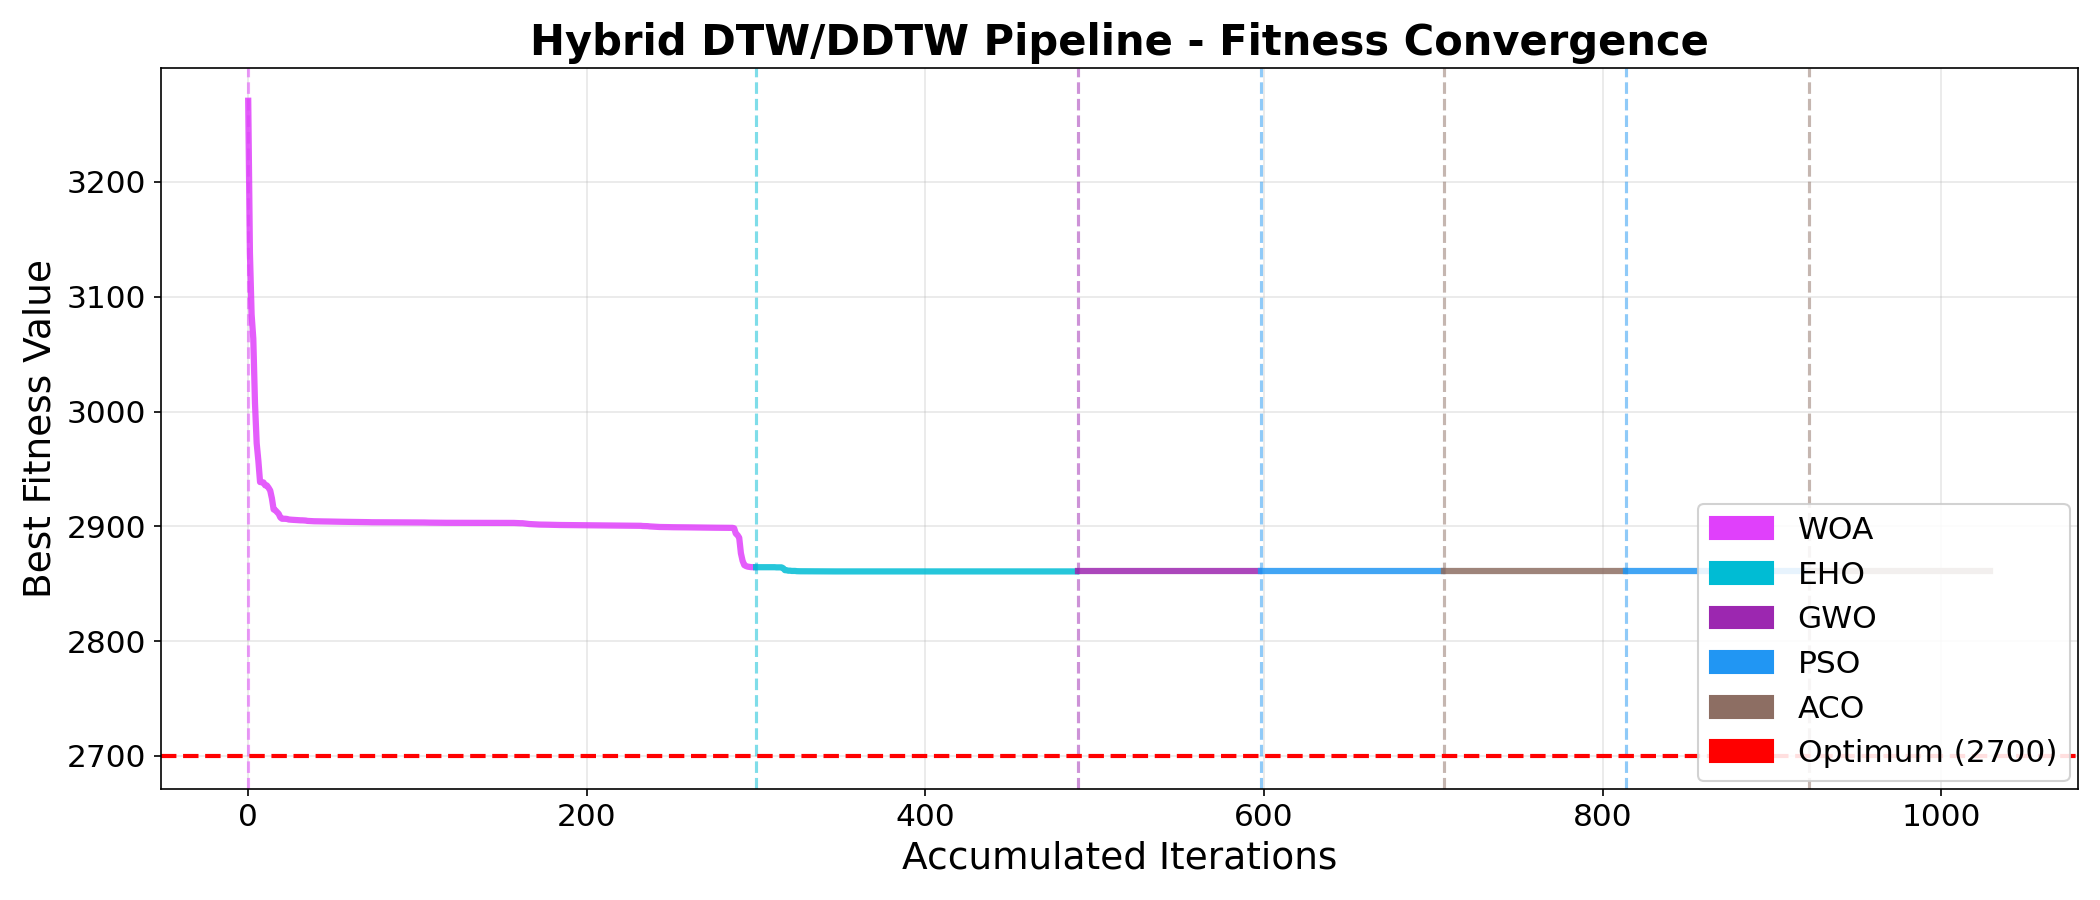
\includegraphics[width=0.7\linewidth]{imagenes_cec_mejores/cec_f12_ddtw_convergencia.png}\hfill
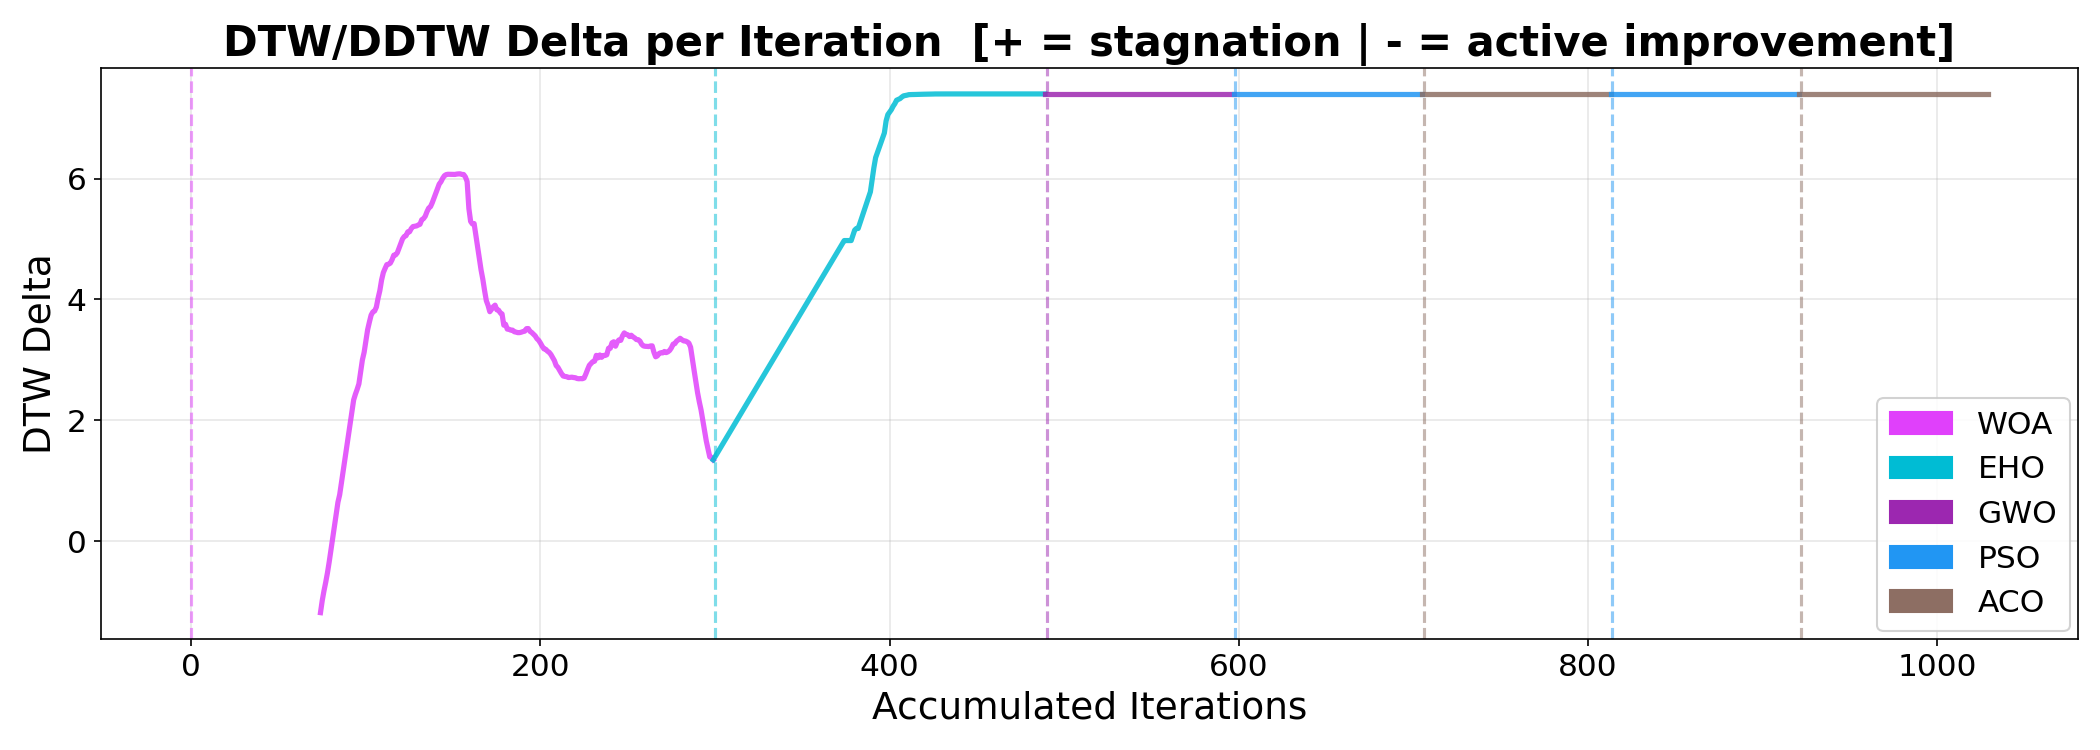
\includegraphics[width=0.7\linewidth]{imagenes_cec_mejores/cec_f12_ddtw_dtw_delta.png}
\caption{Convergence trajectory (left) and $\Delta$ monitor (right) for
\texttt{F12} (Composition Function 4) under DDTW, best run 01.}
\label{fig:cec-best-f12}
\end{figure}
